\chapter{Tidal Disruption of Neutron Stars with Hot, Nuclear Equations of State}
\label{chap:chapter-5}

\section{Initial Configuration}
\label{sec:initial-config}

The models considered in this survey consider those black hole whose Christodoulou mass is $M_{\rm BH} = 7 M_\odot$ with an orbitally-aligned, prograde dimensionless spin of $\chi_{\rm BH} = 0.9$.
The black hole mass is in the range of masses of X-ray binary observations~\cite{Ozel:2010,Kreidberg:2012}, while the spin is chosen to ensure tidal disruption of a neutron star outside the black hole.
We choose a naming scheme such that model M12-M7-S9-FSU21 represents an ADM neutron star mass of $M_{\rm NS} = 1.2 M_\odot$, a black hole of mass and dimensionless spin $M_{\rm BH} = 7 M_\odot$ and $\chi_{\rm BH} = 0.9$, and the FSU2.1 neutron star equation of state.
In Table \ref{tab:id}, we provide a list of the initial values for the models used in this paper.

The TOV equations which govern gravitational equilibrium under general relativity are solved to construct the neutron star in isolation; that is, to produce the initial central density $\rho_c$, neutron star baryon mass $M^b_{\rm NS}$ and radius $R_{\rm NS}$ via a basic root solving technique in density given an available finite-temperature, nuclear theory-based equation of state table.
The neutron star fluid is assumed to be in hydrostatic equilibrium, irrotational, cold ($T = 0.1 {\rm MeV}$) and in $\beta$-equilibrium.
We start with an initial coordinate separation between the two objects that is fairly close ($d \sim 80 {\rm km}$), where the binary is in a quasicircular orbit
(i.e. small eccentricities $e \sim 0.01$).
Ultimately, the equations to be solved in the system are the hydrostatic equilibrium equations in a co-rotating frame of the binary, and the Einstein constraint equations.  
These evolution equations are solved with an in-house elliptic solver in \SpEC, as described in Chapter \ref{chap:chapter-3}.
All models studied here orbit $5 - 6$ times during inspiral, before the neutron star begins to tidally disrupt and accrete onto the black hole.

\begin{table}
	\begin{center}
	\caption[Initial parameters of binaries used in this survey]{
		Initial parameters of the binaries studied in this work. 
		$M_{\rm NS}$ is the ADM mass of an isolated neutron star with the same equation of state and baryon mass as the neutron star under
		consideration, $N_{\rm orbits}$ is the number of orbits up to the point at which $0.01M_\odot$ has been accreted by the black hole,
		$\Omega_0$ is the initial angular velocity, and the system mass is $M=M_{\rm BH}+M_{\rm NS}$. We use the same resolution for each simulation: $\Delta x_{\rm dis} = 160{\rm m}$ is the typical grid resolution in the laboratory frame
		for the finest level of refinement used during the disruption of the neutron star (see Sec.~\ref{sec:hydro-amr} for more detail on the grid structure).}
	\label{tab:id}
	{
		\begin{tabular}{|l||ccccc|}
	%\toprule
	\hline
	Model & $M_{\rm NS}\,(M_\odot)$ & $R_{\rm NS}\,({\rm km})$ & $\cal{C}_{\rm NS}$ & $N_{\rm orbits}$ & $\Omega_0 M$ \\
	%\midrule\midrule
	\hline%\hline
	M12-M7-S9-DD2 & 1.2 & 13.1 & 0.135 & 5.0 & fill1\\
	M14-M7-S9-DD2 & 1.4 & 13.2 & 0.156 & 6.0 & fill1\\
	M12-M7-S9-FSU21 & 1.2 & 13.5 & 0.130 & 4.9 & fill1\\
	M14-M7-S9-FSU21 & 1.4 & 13.6 & 0.152 & 5.5 & fill1\\
	M12-M7-S9-SFHo & 1.2 & 11.9 & 0.148 & 5.3 & fill1\\
	M14-M7-S9-SFHo & 1.4 & 11.8 & 0.173 & 5.9 & fill1\\
	M12-M7-S9-SFHx & 1.2 & 11.9 & 0.149 & 5.2 & fill1\\
	M14-M7-S9-SFHx & 1.4 & 11.9 & 0.173 & 5.4 & fill1\\
%			M12-M7-S9-LS220 & 1.2 & 12.7 & 0.139 & fill0 & fill & 160\\
%			M14-M7-S9-LS220 & 1.4 & 12.6 & 0.163 & fill0 & fill & 170\\
	\hline
	%\bottomrule
\end{tabular}
	}
	\end{center}
\end{table}


\section{Merger dynamics}
\label{sec:merger-dynamics}

All of our models disrupt outside the inner most stable circular orbit of the black hole.  
All of our models were evolved with the same minimum grid spacing of $\Delta x_{\rm dis} = 245{\rm m}$ on the innermost level of refinement, in the grid coordinates.  
In the inertial frame, the average minimum grid spacing is typically around $\sym (150-200)$m during the merger.  
This is because in the grid frame, the grid spacing gets coarser in the direction in which the tidal stream expands and gets finer in the directions it contracts.


\begin{figure}
	\centering
	\begin{subfigure}[b]{0.475\textwidth}
		\centering
		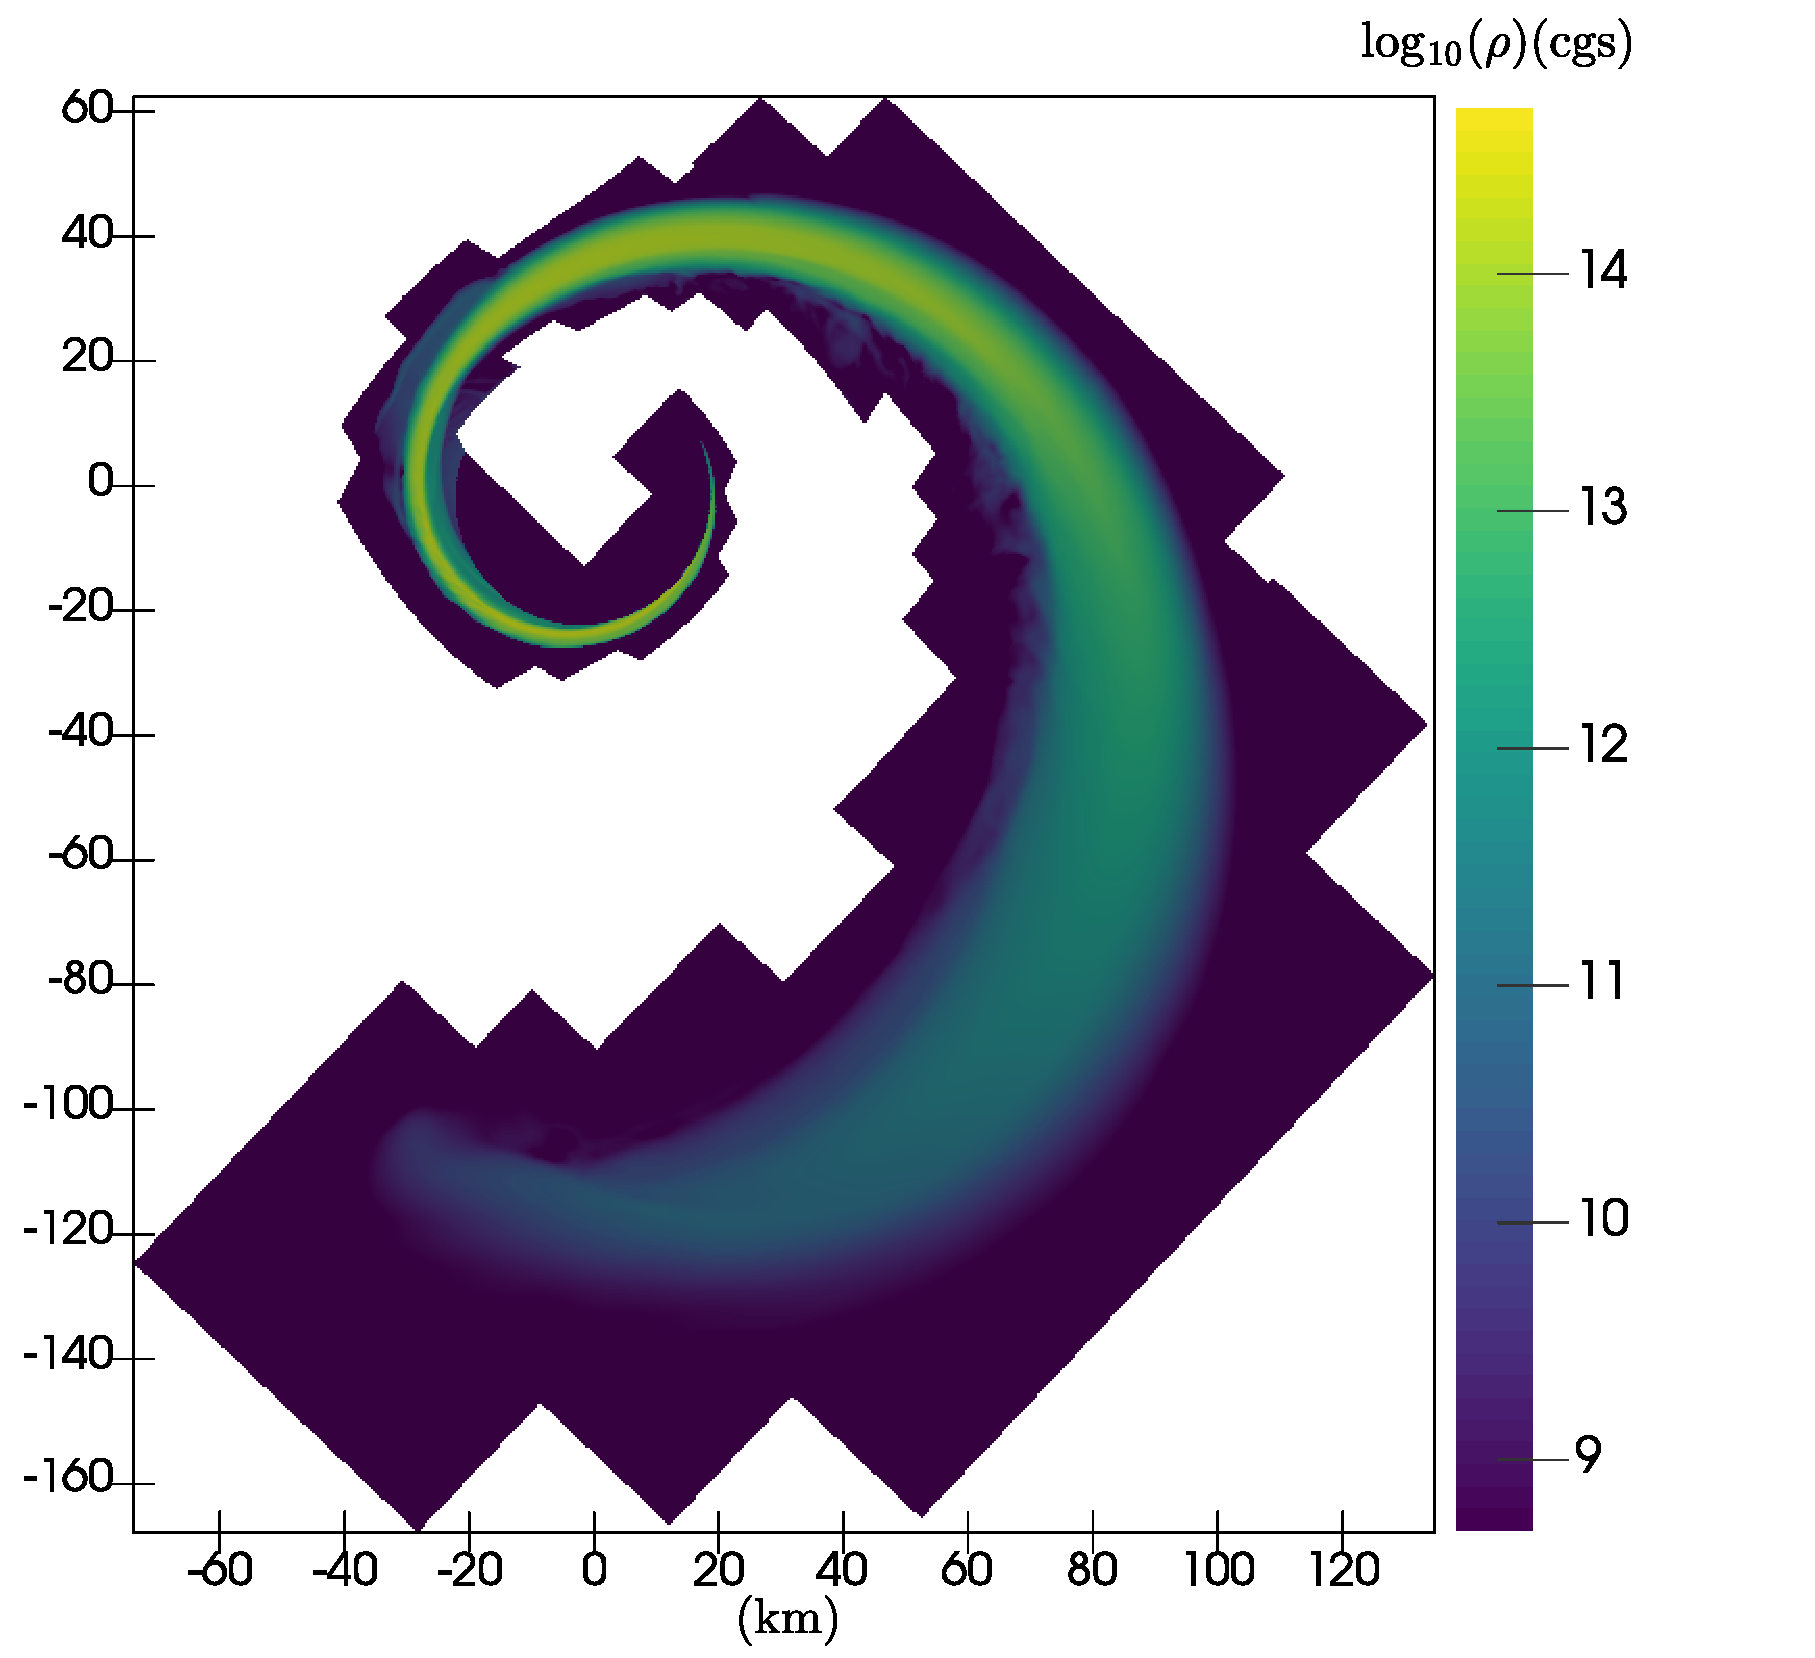
\includegraphics[width=1.0\linewidth]{images/rho_DD2_M12-merger-inertial}
		\label{fig:rho_M12_DD2}
	\end{subfigure}
	\begin{subfigure}[b]{0.475\textwidth}
		\centering
		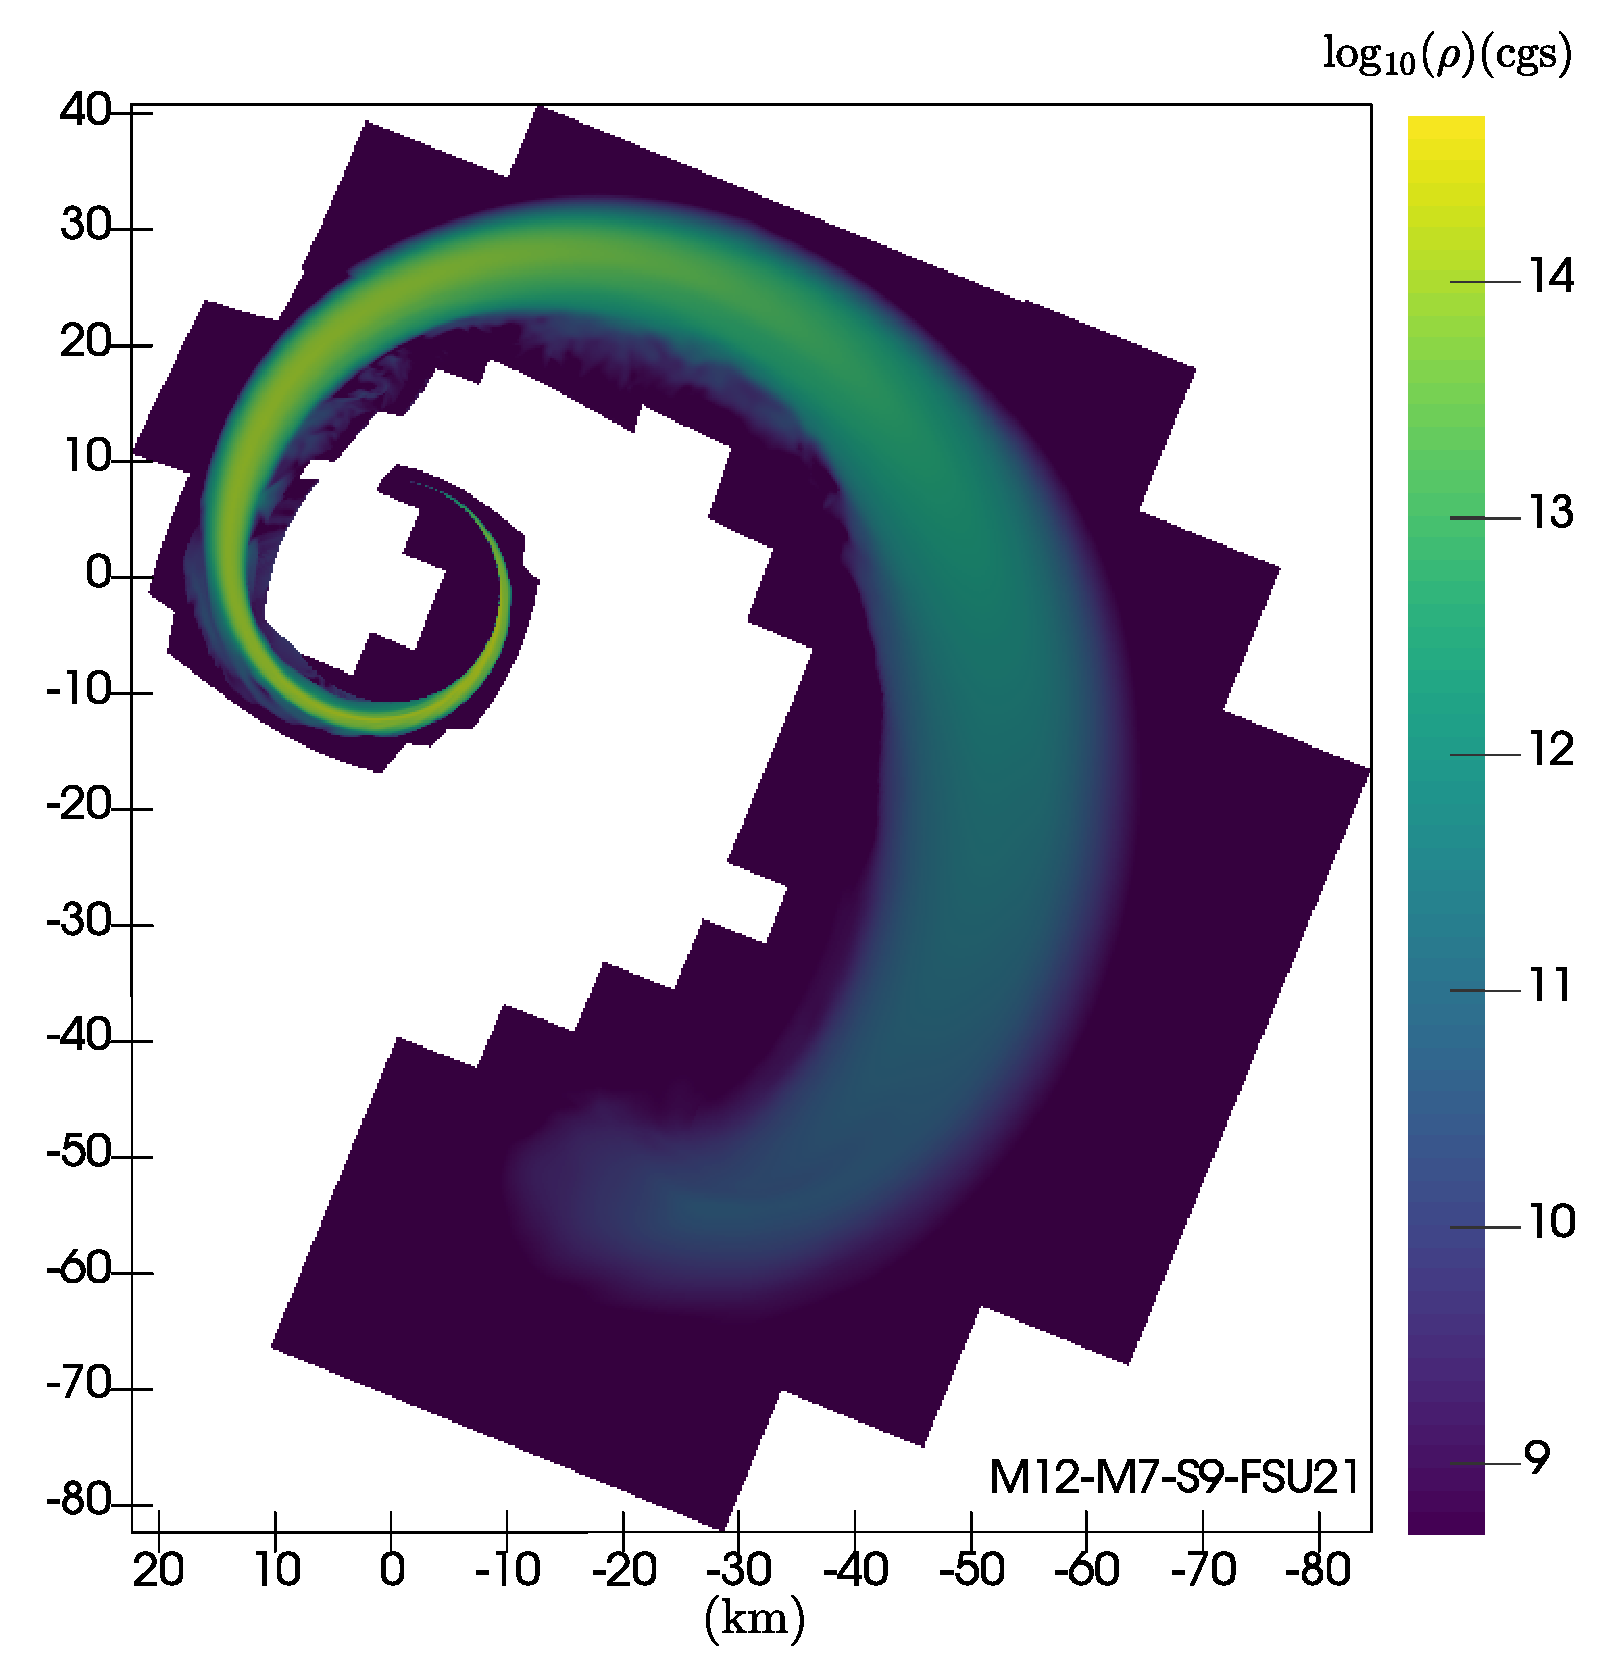
\includegraphics[width=\linewidth]{images/rho_FSU21_M12-merger-inertial}
		\label{fig:rho_M12_FSU21}
	\centering
	\end{subfigure}
	\begin{subfigure}[b]{0.475\textwidth}
		\centering
		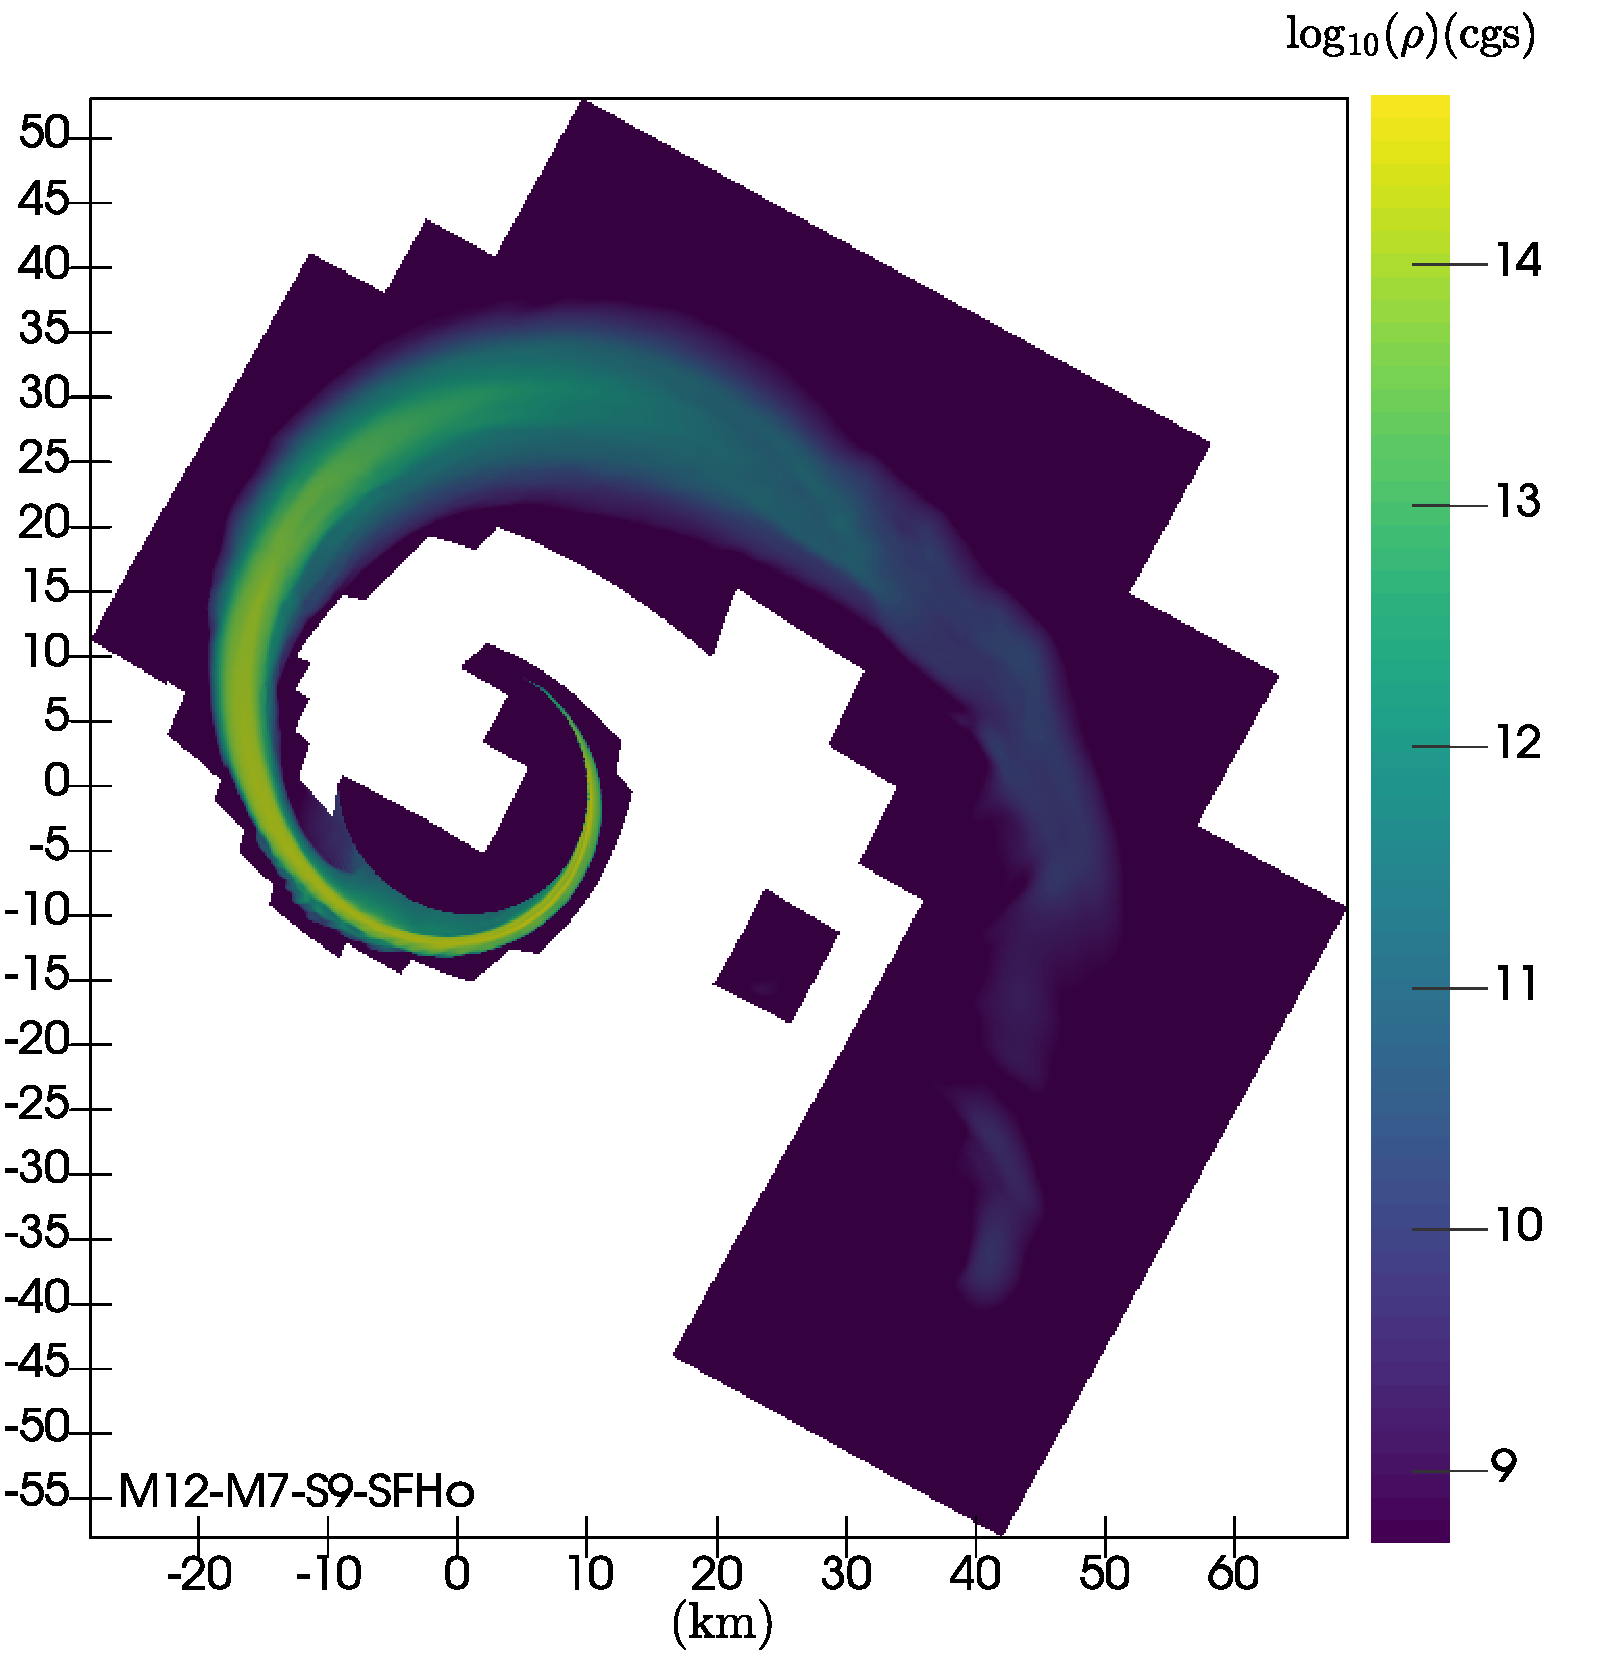
\includegraphics[width=\linewidth]{images/rho_SFHo_M12-merger-inertial}
		\label{fig:rho_M12_SFHo}
	\end{subfigure}
	\begin{subfigure}[b]{0.475\textwidth}
		\centering
		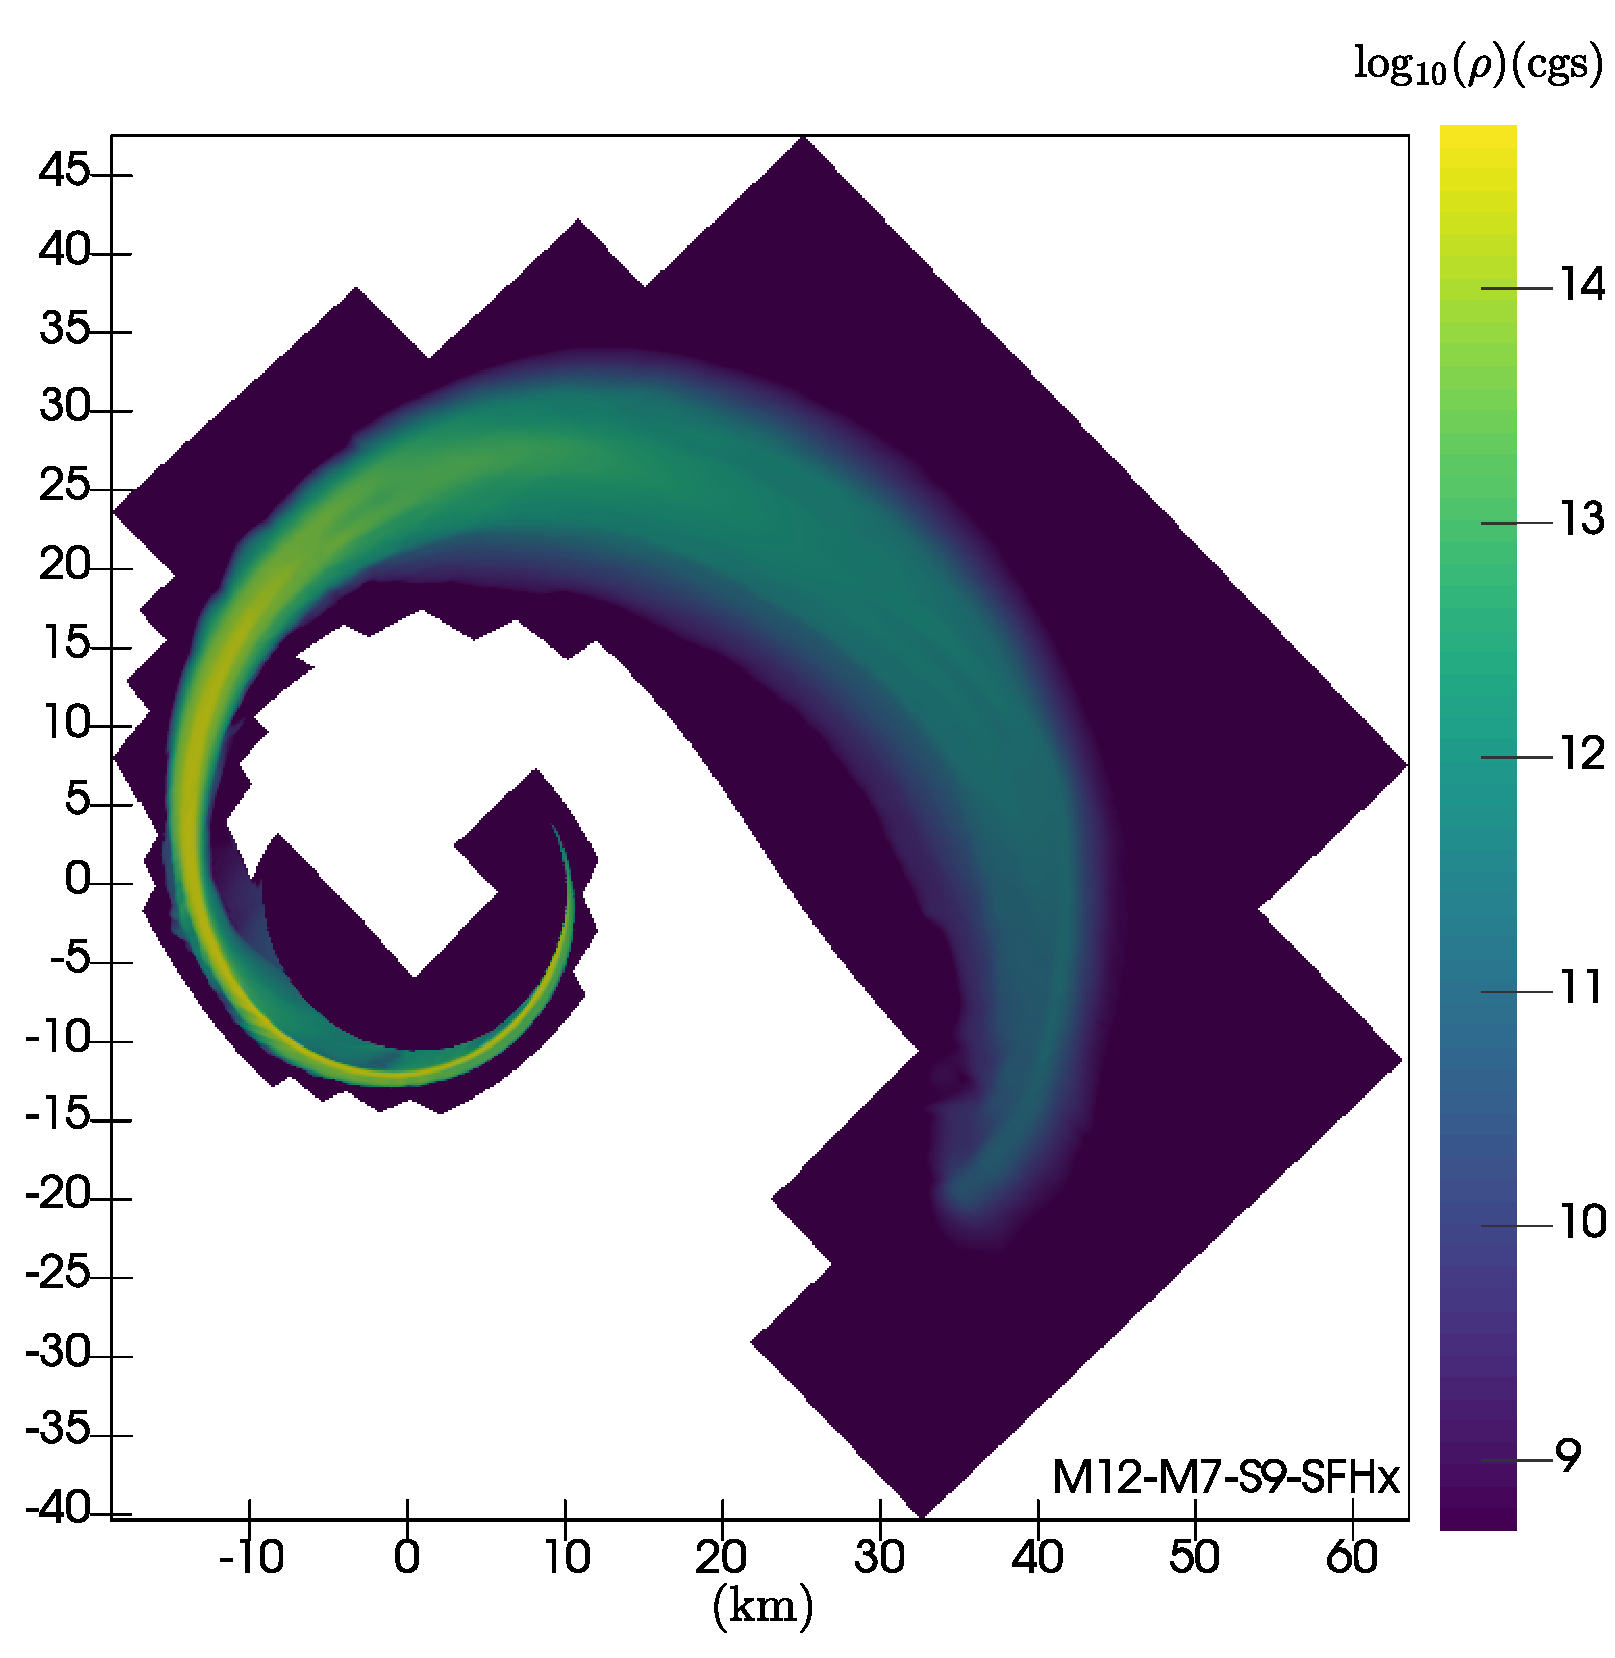
\includegraphics[width=\linewidth]{images/rho_SFHx_M12-merger-inertial}
		\label{fig:rho_M12_SFHx}
	\end{subfigure}
	\caption[Density profiles on equatorial plane for $1.2 M_{\odot}$ models]{
		Baryon density profiles on the equatorial plane for $M_{\rm NS} = 1.2 M_{\odot}$ models when $50\%$ of the neutron star material has been accreted onto the black hole.
		\textit{Top left:} Model M12-M7-S9-DD2.
		\textit{Top right:} Model M12-M7-S9-FSU21.
		\textit{Bottom left:} Model M12-M7-S9-SFHo.
		\textit{Bottom right:} Model M12-M7-S9-SFHx.
		White regions are not covered by the finite volume grid, while some fluid subdomains overlap the excised region of the black hole which can be seen near the interface of inflowing matter and the horizon.  We bracket the baryon density between $\sym \rho_{\rm FMR}$ and the fiducial density, $10^{14.7} {\rm g\,cm^{-3}}$. Note the distortion (and rotation) of the finite volume subdomain boundaries in the finest, innermost level, since the fluid is evolved in the coordinates of the (non-rotating) pseudo-spectral grid and we are viewing the systems in the inertial frame.  Also note the difference in length scales between models at merger time.
	}
	\label{fig:rho_M12}
\end{figure}

In Figure \ref{fig:rho_M12} we show the snapshot of each $1.2 M_\odot$ model on the equatorial plane when 50\% of the neutron star material has been accreted onto the black hole.  
In Figure \ref{fig:rho_M14}, Model M14-M7-S9-FSU21 shows the ``poofiest'' (widest) outer tail, measuring $\sym 20 {\rm km}$ across, while M12-M7-S9-DD2 measures at $\sym 12 {\rm km}$ in breadth.  
The infalling stream near the horizon gets very narrow, and as such caused a number of our softest models to become too difficult to evolve.  
In those cases, the stream overlaps very few points on the finite volume grid, which led to unphysical temperatures and orbital energy buildup.  
Both SFHx
\footnote{
The M12-M7-S9-SFHx model did evolve far enough to get ejecta information, but that run ran into other numerical artifacts after the merger.
}
as well as the M14-M7-S9-SFHo models did not proceed past merger beyond a few fractions of a millisecond.

Consulting Figure \ref{fig:MultGammavsRho}, while all models soften near the fiducial density, the most drastic change in the high-density infalling region occurs in SFHx.  In our studies, the measured average temperature of the soft $1.4 M_\odot$ models was much higher near merger time (at which point the average temperature in all models reaches a maximum), and could indicate that the simulations were poorly resolved, at least in the innermost levels of the finite volume grid.  Therefore, we do not include the snapshots for M14-M7-S9-SFHo of M14-M7-S9-SFHx, while the snapshot for M12-M7-S9-SFHx is only included because it was well-behaved up to merger.

\begin{figure*}
	\centering
	\begin{subfigure}[b]{0.475\textwidth}
		\centering
		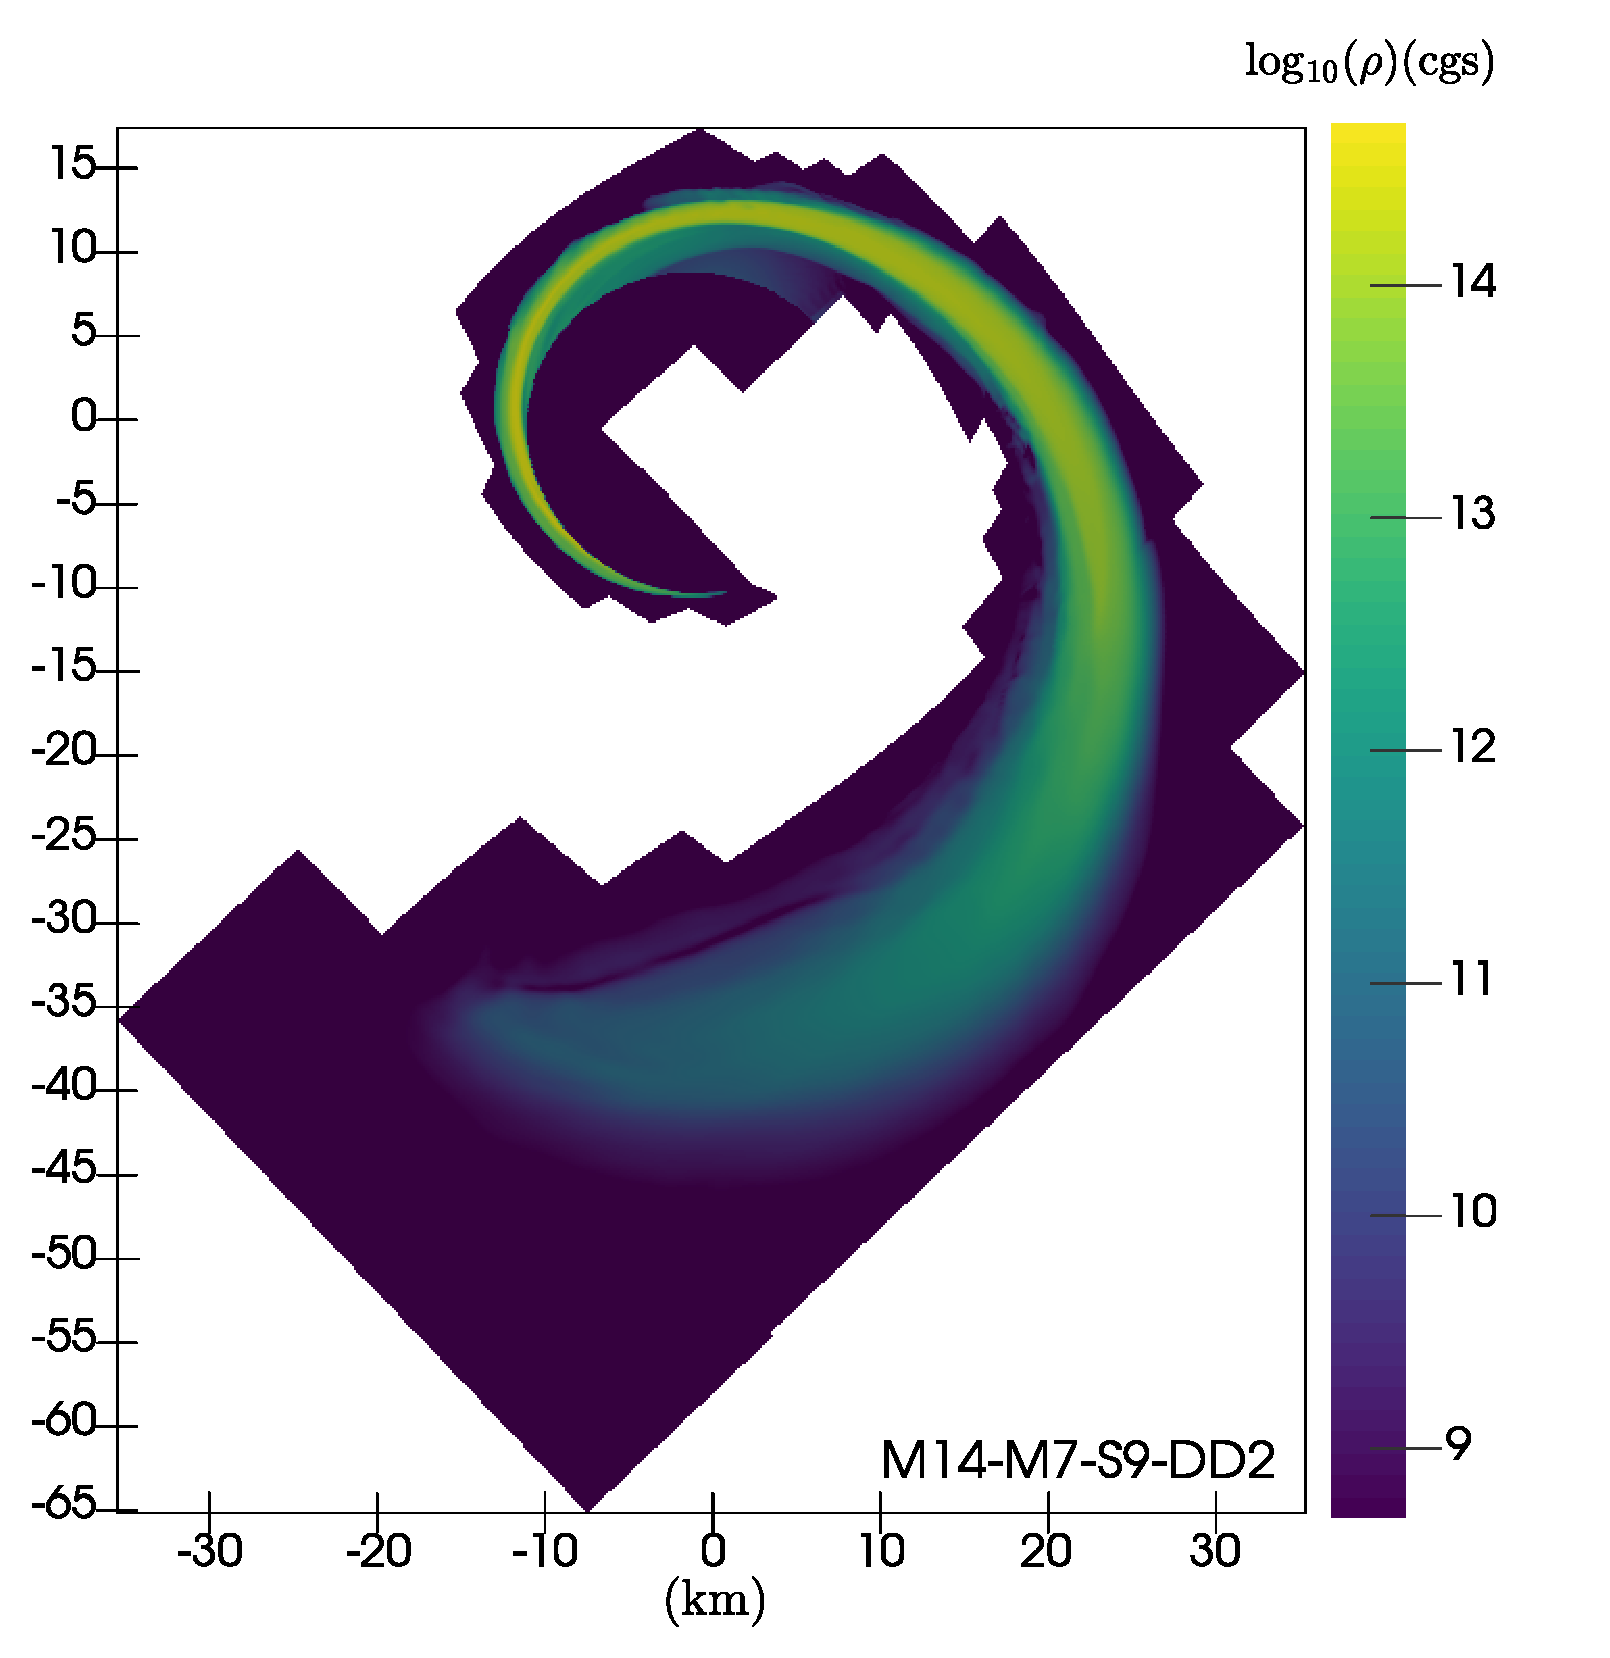
\includegraphics[width=1.0\linewidth]{images/rho_DD2_M14-merger-inertial}
		\label{fig:rho_M14_DD2}
	\end{subfigure}
	\begin{subfigure}[b]{0.475\textwidth}
		\centering
		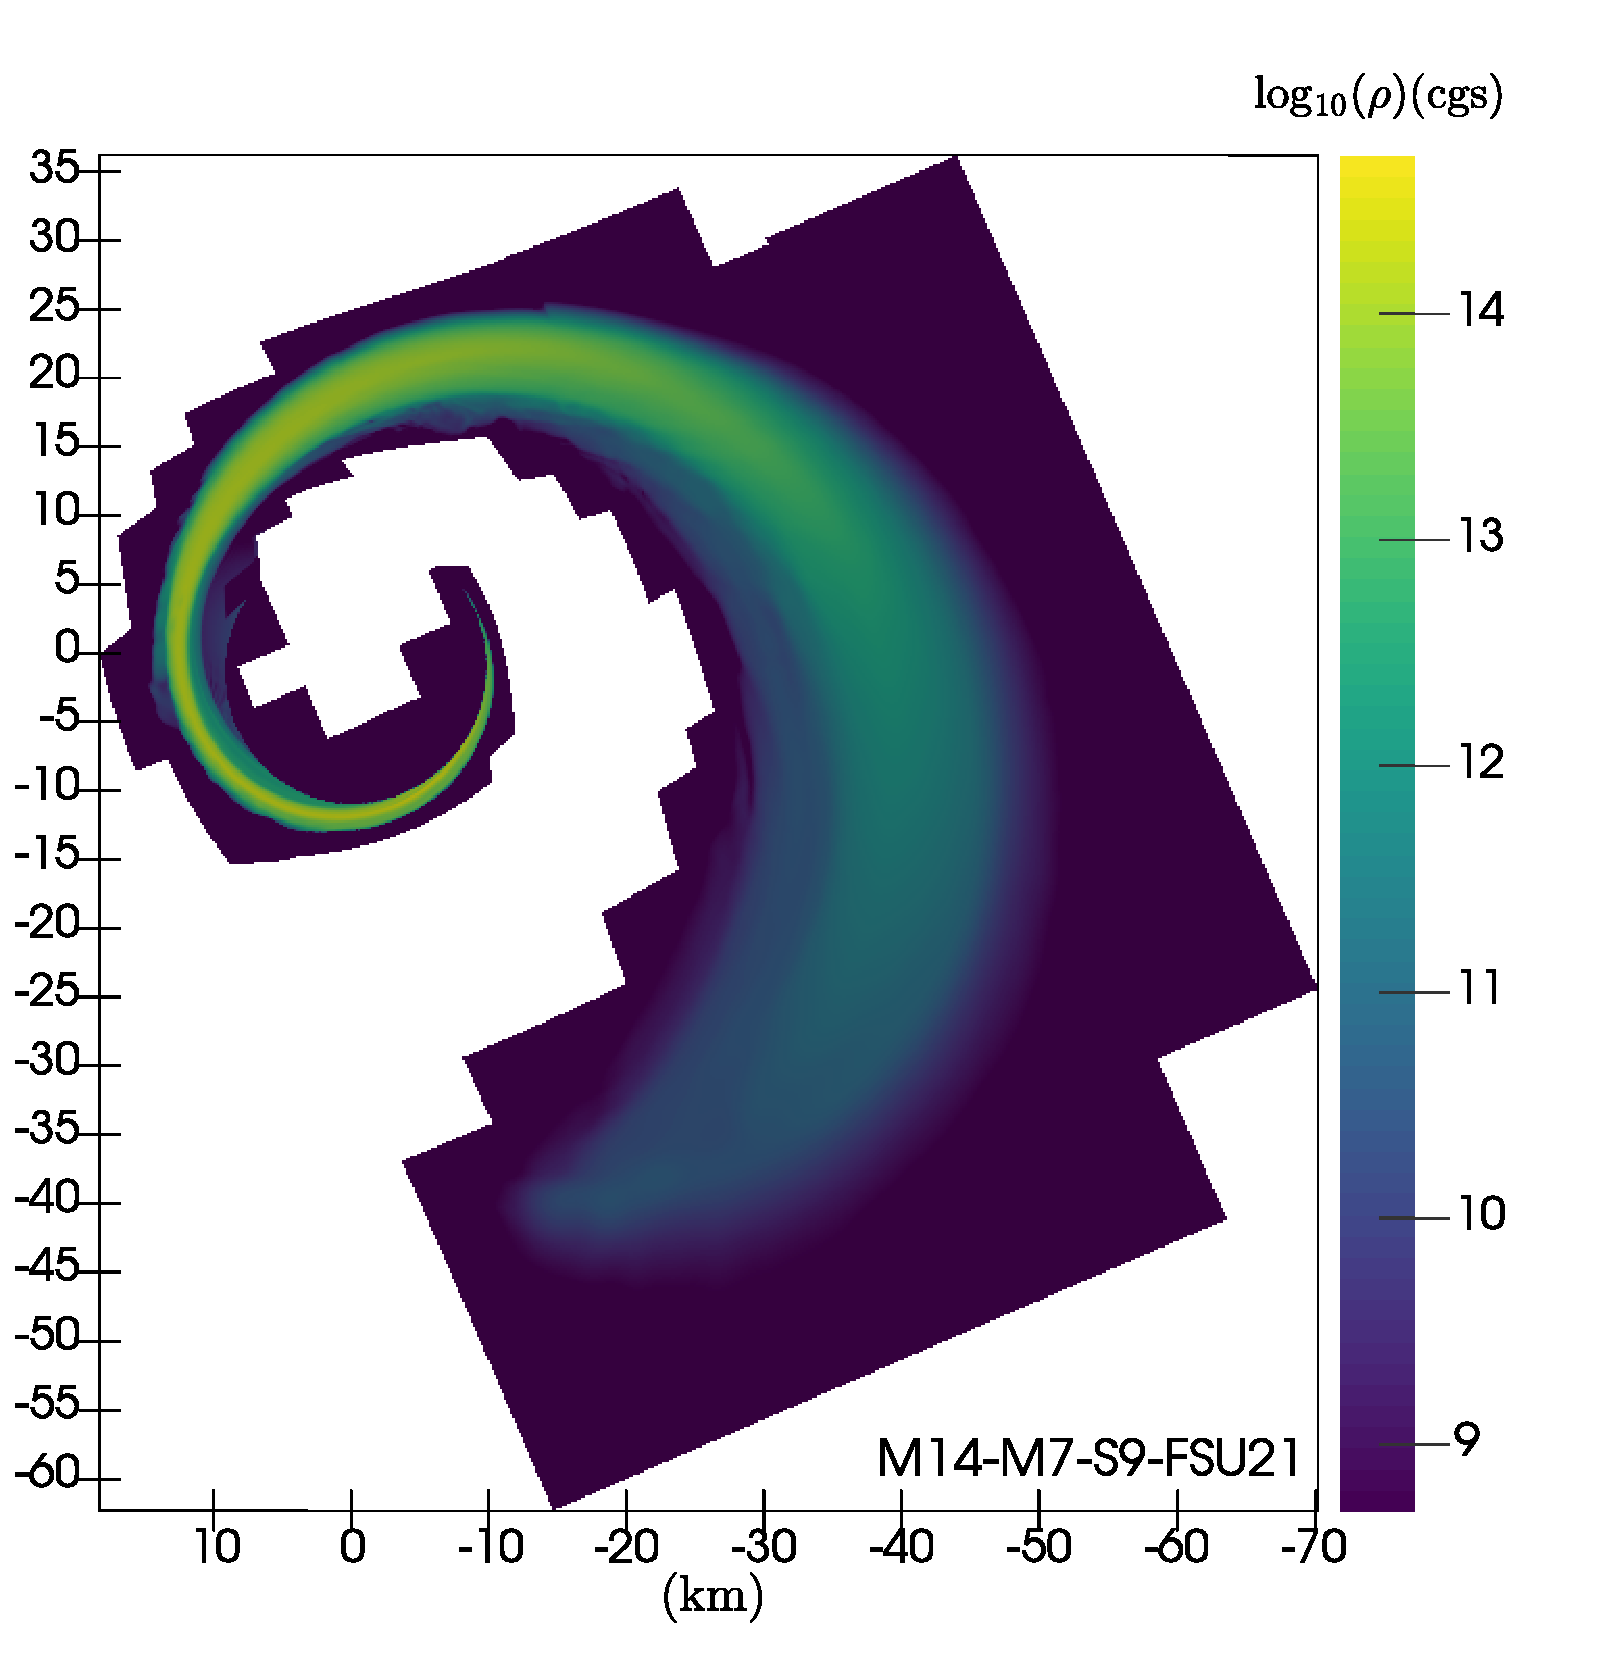
\includegraphics[width=\linewidth]{images/rho_FSU21_M14-merger-inertial}
		\label{fig:rho_M14_FSU21}
		\centering
	\end{subfigure}
	\caption[Density profiles on equatorial plane for $1.4 M_{\odot}$ models]{
	Baryon density profiles on the equatorial plane for $M_{\rm NS} = 1.4 M_{\odot}$ models when $50\%$ of the neutron star material has been accreted onto the black hole.
	\textit{Left:} Model M14-M7-S9-DD2.
	\textit{Right:} Model M14-M7-S9-FSU21.
	To add to the caption in Figure \ref{fig:rho_M12}, we note that the FSU2.1 profiles are represented with a $90^{\circ}$ counterclockwise rotation in the inertial frame.  This is done for sake of maintaining a similar aspect ratio to the others.  Note that FSU2.1 had the fewest number of orbits in our simulations (see Table \ref{tab:id}). 
	}
	\label{fig:rho_M14}
\end{figure*}

Shortly after the merger, between the time at which we define as when 50\% of the neutron star mass has been deposited on the black hole, and the first local minimum of the accretion rate and average temperature, we derefine the innermost finite volume level by a factor of two.
The fluid begins to circularize $\sym (3-4) {\rm ms}$ after merger in all models.
We perform a second derefinement by a factor of two more at 
this stage as well, since the material becomes less dense and easier to resolve.



\begin{table}
	\begin{center}
		\caption[Properties of the dynamical ejecta and post merger remnant]{
			Properties of the dynamical ejecta and post merger remnant. $M_{\rm BH}^f$ and  $\chi_{\rm BH}^f$  are the mass and dimensionless spin of the black hole,
			and $M_{\rm out}^f$ is the baryon mass remaining outside of the black hole. Those quantities are measured at the first minima of the accretion rate onto the black hole,
			before circularization of the accretion disk. The baryon mass outside of the black hole immediately after disk formation (which is a more vaguely defined
			time) is typically $10\%-20\%$ lower than $M_{\rm out}^f$. $M_{\rm ej}$ is the mass of the dynamical ejecta, and $\langle v/c\rangle_{\rm ej}$. All these properties are nearly constant, from about $1\,{\rm ms}$ after the merger. Bracketed numbers for
			$M_{\rm out}^f$ and $M_{\rm ej}$ show semi-analytical predictions for the mass outside of the black hole $10\,{\rm ms}$ after merger~\cite{Foucart2012},
			and the ejected mass~\cite{Kawaguchi:2016}, while bracketed numbers for $M_{\rm BH}^f$ and $\chi_{\rm BH}^f$ are semi-analytical predictions
			from~\cite{Pannarale:2014}. Those values were calculated from the equations in~\cite{Pannarale:2014} using a root-finding code for both the innermost stable spherical orbit and the reported quantities.  Relative errors in the determination of $M_{\rm ej}$ are $\sim 20\%$, the black holes properties are
			accurate to $\sim 1\%$, and other quantities have relative errors of $\sim 10\%$.
		}
		\label{tab:results}
		{
			\begin{tabular}{c cc ccc}
	\toprule \toprule
	Model & $M_{\rm BH}^f\,(M_\odot)$ & $\chi_{\rm BH}^f$ & $M_{\rm out}^f\,(10^{-2} M_\odot)$ & $M_{\rm ej}\,(10^{-2} M_\odot)$ & $\langle v/c \rangle_{\rm ej}$\\
	\midrule
	M12-M7-S9-DD2 & -- [7.7] & -- [0.93] & -- [36] & 7.2 [7.2] & 0.21\\
	M14-M7-S9-DD2 & -- [7.9] & -- [0.93] & -- [34] & 6.0 [3.6] & 0.20\\
	M12-M7-S9-FSU21 & -- [7.7] & -- [0.93] & -- [38] & 7.8 [10.7] & 0.20\\
	M14-M7-S9-FSU21 & -- [7.9] & -- [0.93] & -- [36] & 5.9 [6.4] & 0.19\\
	M12-M7-S9-SFHo & -- [7.8] & -- [0.93] & -- [30] & $\sym 3.8$ [4.3] & $\sym 0.18$\\
	M14-M7-S9-SFHo & -- [8.0] & -- [0.93] & -- [26] & -- [2.3] & --\\
	M12-M7-S9-SFHx & -- [7.8] & -- [0.93] & -- [30] & $\sym 5.7$ [5.9] & $\sym0.20 $\\
	M14-M7-S9-SFHx & -- [8.0] & -- [0.93] & -- [26] & -- [2.6] & --\\
%	M12-M7-S9-LS220 & -- [7.8] & -- [0.93] & -- [34] & -- [9.4] & --\\
%	M14-M7-S9-LS220 & -- [8.0] & -- [0.93] & -- [31] & -- [4.7] & --\\
	\bottomrule \bottomrule
\end{tabular}
		}
	\end{center}
\end{table}



\section{Outflow analysis: properties of the ejecta}
\label{sec:tail-analysis}

In this section, we consider the ejecta that results from the tidal disruption of the neutron star, leaving aside the second source of late-stage ejecta which occurs via neutrino driven winds and magnetic effects in accretion disk outlfows.  
As our models do not incorporate magnetohydrodynamics and since we only implement a simple leakage scheme to approximately capture the effects of neutrino cooling on the post-merger disk of Section \ref{sec:disk-analysis}, we do not evolve the remaining models beyond $10 {\rm ms}$ passed the onset of merger.
On the other hand, the dynamical unbound ejecta leaves the system before strong heating occurs, so not much neutrino processing is expected, and the lack of neutrino transport is probably not much of a problem.
This is in contrast to the double neutron star ejecta, where effects of neutrino absorbtion on ejecta composition is known to be large.

For those models that evolved out to $5 {\rm ms}$ passed merger 
(a reasonable time to choose, since this is more than enough time for the motion to become ballistic and reported quantities to settle from the ejecta),
we find that at that time, the ejecta mass $M_{\rm ej}$ is constrained between $\sym (4 - 8) \times 10^{-2} M_\odot$.
In table \ref{tab:results}, we display our measured results at $5 {\rm ms}$ after measure (at this time the ejecta has leveled off for $\gtrsim 2$ms) compared to the predicted results from the fitting formulae.  
As described by the fitting formulae, the stiffer equations of state do indeed disrupt further outside the ISCO, while the softer one disrupts much closer and results in more interaction between the protodisk and the fallback material.


\begin{figure}
	\centering
	% GNUPLOT: LaTeX picture with Postscript
\begingroup
  \makeatletter
  \providecommand\color[2][]{%
    \GenericError{(gnuplot) \space\space\space\@spaces}{%
      Package color not loaded in conjunction with
      terminal option `colourtext'%
    }{See the gnuplot documentation for explanation.%
    }{Either use 'blacktext' in gnuplot or load the package
      color.sty in LaTeX.}%
    \renewcommand\color[2][]{}%
  }%
  \providecommand\includegraphics[2][]{%
    \GenericError{(gnuplot) \space\space\space\@spaces}{%
      Package graphicx or graphics not loaded%
    }{See the gnuplot documentation for explanation.%
    }{The gnuplot epslatex terminal needs graphicx.sty or graphics.sty.}%
    \renewcommand\includegraphics[2][]{}%
  }%
  \providecommand\rotatebox[2]{#2}%
  \@ifundefined{ifGPcolor}{%
    \newif\ifGPcolor
    \GPcolortrue
  }{}%
  \@ifundefined{ifGPblacktext}{%
    \newif\ifGPblacktext
    \GPblacktexttrue
  }{}%
  % define a \g@addto@macro without @ in the name:
  \let\gplgaddtomacro\g@addto@macro
  % define empty templates for all commands taking text:
  \gdef\gplbacktext{}%
  \gdef\gplfronttext{}%
  \makeatother
  \ifGPblacktext
    % no textcolor at all
    \def\colorrgb#1{}%
    \def\colorgray#1{}%
  \else
    % gray or color?
    \ifGPcolor
      \def\colorrgb#1{\color[rgb]{#1}}%
      \def\colorgray#1{\color[gray]{#1}}%
      \expandafter\def\csname LTw\endcsname{\color{white}}%
      \expandafter\def\csname LTb\endcsname{\color{black}}%
      \expandafter\def\csname LTa\endcsname{\color{black}}%
      \expandafter\def\csname LT0\endcsname{\color[rgb]{1,0,0}}%
      \expandafter\def\csname LT1\endcsname{\color[rgb]{0,1,0}}%
      \expandafter\def\csname LT2\endcsname{\color[rgb]{0,0,1}}%
      \expandafter\def\csname LT3\endcsname{\color[rgb]{1,0,1}}%
      \expandafter\def\csname LT4\endcsname{\color[rgb]{0,1,1}}%
      \expandafter\def\csname LT5\endcsname{\color[rgb]{1,1,0}}%
      \expandafter\def\csname LT6\endcsname{\color[rgb]{0,0,0}}%
      \expandafter\def\csname LT7\endcsname{\color[rgb]{1,0.3,0}}%
      \expandafter\def\csname LT8\endcsname{\color[rgb]{0.5,0.5,0.5}}%
    \else
      % gray
      \def\colorrgb#1{\color{black}}%
      \def\colorgray#1{\color[gray]{#1}}%
      \expandafter\def\csname LTw\endcsname{\color{white}}%
      \expandafter\def\csname LTb\endcsname{\color{black}}%
      \expandafter\def\csname LTa\endcsname{\color{black}}%
      \expandafter\def\csname LT0\endcsname{\color{black}}%
      \expandafter\def\csname LT1\endcsname{\color{black}}%
      \expandafter\def\csname LT2\endcsname{\color{black}}%
      \expandafter\def\csname LT3\endcsname{\color{black}}%
      \expandafter\def\csname LT4\endcsname{\color{black}}%
      \expandafter\def\csname LT5\endcsname{\color{black}}%
      \expandafter\def\csname LT6\endcsname{\color{black}}%
      \expandafter\def\csname LT7\endcsname{\color{black}}%
      \expandafter\def\csname LT8\endcsname{\color{black}}%
    \fi
  \fi
  \setlength{\unitlength}{0.0500bp}%
  \begin{picture}(7920.00,5040.00)%
    \gplgaddtomacro\gplbacktext{%
      \csname LTb\endcsname%
      \put(1342,704){\makebox(0,0)[r]{\strut{} 1e-07}}%
      \put(1342,1383){\makebox(0,0)[r]{\strut{} 1e-06}}%
      \put(1342,2061){\makebox(0,0)[r]{\strut{} 1e-05}}%
      \put(1342,2740){\makebox(0,0)[r]{\strut{} 0.0001}}%
      \put(1342,3418){\makebox(0,0)[r]{\strut{} 0.001}}%
      \put(1342,4097){\makebox(0,0)[r]{\strut{} 0.01}}%
      \put(1342,4775){\makebox(0,0)[r]{\strut{} 0.1}}%
      \put(1474,484){\makebox(0,0){\strut{} 0}}%
      \put(2684,484){\makebox(0,0){\strut{} 0.05}}%
      \put(3894,484){\makebox(0,0){\strut{} 0.1}}%
      \put(5103,484){\makebox(0,0){\strut{} 0.15}}%
      \put(6313,484){\makebox(0,0){\strut{} 0.2}}%
      \put(7523,484){\makebox(0,0){\strut{} 0.25}}%
      \put(176,2739){\rotatebox{-270}{\makebox(0,0){\strut{}$\log_{10}(M_{\rm ej})$ ($M_{\odot}$)}}}%
      \put(4498,154){\makebox(0,0){\strut{}$ Y_e $}}%
    }%
    \gplgaddtomacro\gplfronttext{%
      \csname LTb\endcsname%
      \put(6536,4602){\makebox(0,0)[r]{\strut{}M12-M7-S9-DD2}}%
      \csname LTb\endcsname%
      \put(6536,4382){\makebox(0,0)[r]{\strut{}M14-M7-S9-DD2}}%
      \csname LTb\endcsname%
      \put(6536,4162){\makebox(0,0)[r]{\strut{}M12-M7-S9-FSU21}}%
      \csname LTb\endcsname%
      \put(6536,3942){\makebox(0,0)[r]{\strut{}M14-M7-S9-FSU21}}%
      \csname LTb\endcsname%
      \put(6536,3722){\makebox(0,0)[r]{\strut{}M12-M7-S9-SFHo}}%
    }%
    \gplbacktext
    \put(0,0){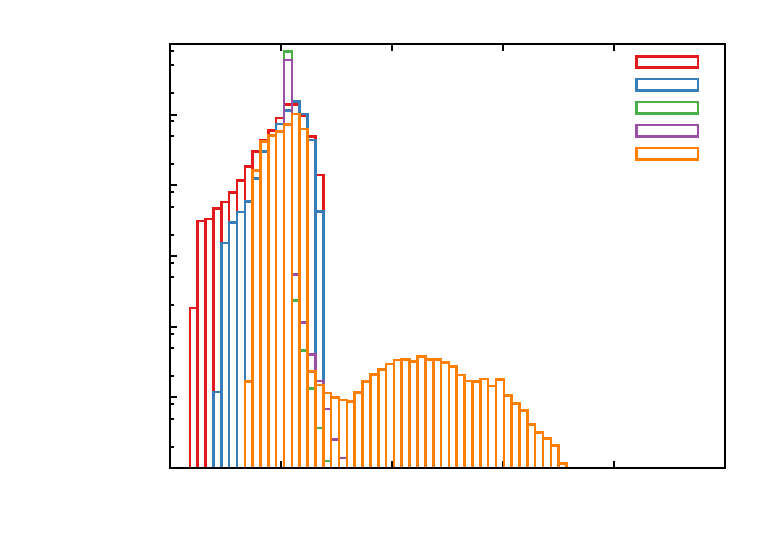
\includegraphics{images/unbound-mass-vs-Ye}}%
    \gplfronttext
  \end{picture}%
\endgroup

	\caption[Composition of the ejecta]{
		Electron fraction $Y_e$ of the ejecta measured 5 ms after merger.  
		We note that all of the matter peaks in the $Y_e \sym 0.05$ range, where M12-M7-S9-DD2 has the largest electron fraction range ($0.011 - 0.07$) while neither FSU21 models produce ejecta with $Y_e < 0.05$. 
		(FSU2.1 does not allow for $Y_e < 0.05$.  See Section \ref{sec:fsu21} and ~\cite{shen2011second}).
	}
	\label{fig:Yehisto}
\end{figure}

As in our previous simulations of black hole-neutron star mergers, the ejecta in our models is very neutron rich, with a density-weighted average electron fraction of $Y_e \sim 0.05$).  
In Figure \ref{fig:Yehisto}, we show the (logarithmic) distribution of matter over the chemical composition in the unbound material.  
Most of the ejecta has $Y_e \lesssim 0.07$ while none of it has $Y_e > 0.25$ --- where lighter r-process elements might be produced.  
Model M12-M7-S9-SFHo has some amount of low-mass matter with intermediate $Y_e$, but it is still small. 
Therefore, r-process nucleosynthesis will produce 2nd and 3rd peak heavy elements in the ejecta, with little production of light elements in the 1st peak~\cite{Lippuner2015}.  
The unbound material will be very opaque, leading to an electromagnetic transient to peak in the infrared~\cite{2013ApJ...775...18B}.

\begin{figure}
	\centering
	% GNUPLOT: LaTeX picture with Postscript
\begingroup
  \makeatletter
  \providecommand\color[2][]{%
    \GenericError{(gnuplot) \space\space\space\@spaces}{%
      Package color not loaded in conjunction with
      terminal option `colourtext'%
    }{See the gnuplot documentation for explanation.%
    }{Either use 'blacktext' in gnuplot or load the package
      color.sty in LaTeX.}%
    \renewcommand\color[2][]{}%
  }%
  \providecommand\includegraphics[2][]{%
    \GenericError{(gnuplot) \space\space\space\@spaces}{%
      Package graphicx or graphics not loaded%
    }{See the gnuplot documentation for explanation.%
    }{The gnuplot epslatex terminal needs graphicx.sty or graphics.sty.}%
    \renewcommand\includegraphics[2][]{}%
  }%
  \providecommand\rotatebox[2]{#2}%
  \@ifundefined{ifGPcolor}{%
    \newif\ifGPcolor
    \GPcolortrue
  }{}%
  \@ifundefined{ifGPblacktext}{%
    \newif\ifGPblacktext
    \GPblacktexttrue
  }{}%
  % define a \g@addto@macro without @ in the name:
  \let\gplgaddtomacro\g@addto@macro
  % define empty templates for all commands taking text:
  \gdef\gplbacktext{}%
  \gdef\gplfronttext{}%
  \makeatother
  \ifGPblacktext
    % no textcolor at all
    \def\colorrgb#1{}%
    \def\colorgray#1{}%
  \else
    % gray or color?
    \ifGPcolor
      \def\colorrgb#1{\color[rgb]{#1}}%
      \def\colorgray#1{\color[gray]{#1}}%
      \expandafter\def\csname LTw\endcsname{\color{white}}%
      \expandafter\def\csname LTb\endcsname{\color{black}}%
      \expandafter\def\csname LTa\endcsname{\color{black}}%
      \expandafter\def\csname LT0\endcsname{\color[rgb]{1,0,0}}%
      \expandafter\def\csname LT1\endcsname{\color[rgb]{0,1,0}}%
      \expandafter\def\csname LT2\endcsname{\color[rgb]{0,0,1}}%
      \expandafter\def\csname LT3\endcsname{\color[rgb]{1,0,1}}%
      \expandafter\def\csname LT4\endcsname{\color[rgb]{0,1,1}}%
      \expandafter\def\csname LT5\endcsname{\color[rgb]{1,1,0}}%
      \expandafter\def\csname LT6\endcsname{\color[rgb]{0,0,0}}%
      \expandafter\def\csname LT7\endcsname{\color[rgb]{1,0.3,0}}%
      \expandafter\def\csname LT8\endcsname{\color[rgb]{0.5,0.5,0.5}}%
    \else
      % gray
      \def\colorrgb#1{\color{black}}%
      \def\colorgray#1{\color[gray]{#1}}%
      \expandafter\def\csname LTw\endcsname{\color{white}}%
      \expandafter\def\csname LTb\endcsname{\color{black}}%
      \expandafter\def\csname LTa\endcsname{\color{black}}%
      \expandafter\def\csname LT0\endcsname{\color{black}}%
      \expandafter\def\csname LT1\endcsname{\color{black}}%
      \expandafter\def\csname LT2\endcsname{\color{black}}%
      \expandafter\def\csname LT3\endcsname{\color{black}}%
      \expandafter\def\csname LT4\endcsname{\color{black}}%
      \expandafter\def\csname LT5\endcsname{\color{black}}%
      \expandafter\def\csname LT6\endcsname{\color{black}}%
      \expandafter\def\csname LT7\endcsname{\color{black}}%
      \expandafter\def\csname LT8\endcsname{\color{black}}%
    \fi
  \fi
  \setlength{\unitlength}{0.0500bp}%
  \begin{picture}(7920.00,5040.00)%
    \gplgaddtomacro\gplbacktext{%
      \csname LTb\endcsname%
      \put(1210,704){\makebox(0,0)[r]{\strut{} 0}}%
      \put(1210,1609){\makebox(0,0)[r]{\strut{} 0.001}}%
      \put(1210,2513){\makebox(0,0)[r]{\strut{} 0.002}}%
      \put(1210,3418){\makebox(0,0)[r]{\strut{} 0.003}}%
      \put(1210,4323){\makebox(0,0)[r]{\strut{} 0.004}}%
      \put(1342,484){\makebox(0,0){\strut{} 0}}%
      \put(2578,484){\makebox(0,0){\strut{} 0.1}}%
      \put(3814,484){\makebox(0,0){\strut{} 0.2}}%
      \put(5051,484){\makebox(0,0){\strut{} 0.3}}%
      \put(6287,484){\makebox(0,0){\strut{} 0.4}}%
      \put(7523,484){\makebox(0,0){\strut{} 0.5}}%
      \put(176,2739){\rotatebox{-270}{\makebox(0,0){\strut{}$M_{\rm ej}$ ($M_{\odot}$)}}}%
      \put(4432,154){\makebox(0,0){\strut{}$ v_r/c $}}%
    }%
    \gplgaddtomacro\gplfronttext{%
      \csname LTb\endcsname%
      \put(6536,4602){\makebox(0,0)[r]{\strut{}M12-M7-S9-DD2}}%
      \csname LTb\endcsname%
      \put(6536,4382){\makebox(0,0)[r]{\strut{}M14-M7-S9-DD2}}%
      \csname LTb\endcsname%
      \put(6536,4162){\makebox(0,0)[r]{\strut{}M12-M7-S9-FSU21}}%
      \csname LTb\endcsname%
      \put(6536,3942){\makebox(0,0)[r]{\strut{}M14-M7-S9-FSU21}}%
      \csname LTb\endcsname%
      \put(6536,3722){\makebox(0,0)[r]{\strut{}M12-M7-S9-SFHo}}%
    }%
    \gplbacktext
    \put(0,0){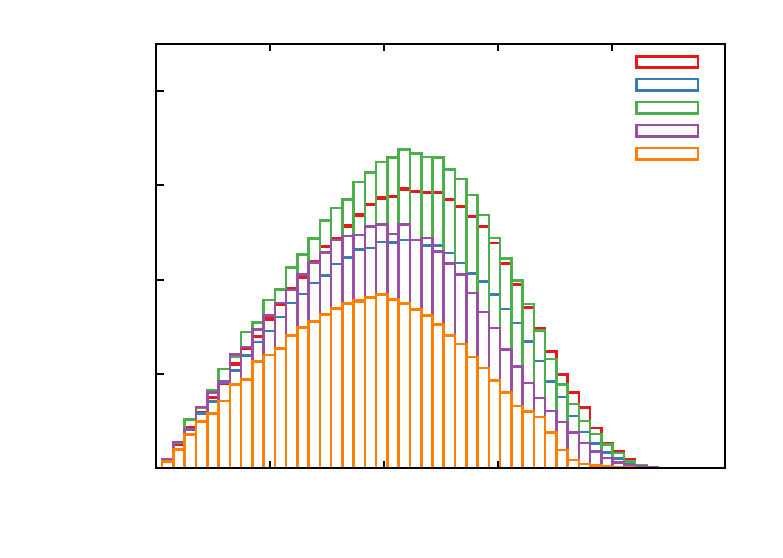
\includegraphics{images/unbound-mass-vs-Vinf}}%
    \gplfronttext
  \end{picture}%
\endgroup

	\caption[Distribution of the asymptotic velocity of the ejecta]{
		Distribution of the asymptotic velocity of the ejecta measured 5 ms after merger.
	}
	\label{fig:vrhisto}
\end{figure}

We can also determine information about the infrared transient from the asymptotic velocity of the ejecta.  
Since greater velocities lead to faster expansion of the unbound material, the transient will be be shorter lived and have a larger amplitude~\cite{2013ApJ...775...18B,Barnes:2016}. 
In Figure \ref{fig:vrhisto}, the distribution of the ejecta velocities peak around $\langle v \rangle \sim 0.2 c$, with a broad distribution  $ 0 \le v \le 2 \langle v \rangle $.
Model M12-M7-S9-SFHo clearly has the least amount of ejecta.

The average kinetic energy of the ejecta was measured to lie between $3.7 \times 10^{52} {\rm ergs} $ for the SFHo model and $4.8 \times 10^{52} {\rm ergs} $ for the M12-M7-S9-DD2 model.  
The $1.4 M_\odot$ models had energies inside this range. 
The ejecta steadily cools within 1 ms after merger to a steady temperature in the range of $T \sim (0.1 - 0.4) {\rm MeV}$, bounded by both FSU2.1 models in the higher range and the remaining models in the lower range.

\begin{figure}
	\centering
	% GNUPLOT: LaTeX picture with Postscript
\begingroup
  \makeatletter
  \providecommand\color[2][]{%
    \GenericError{(gnuplot) \space\space\space\@spaces}{%
      Package color not loaded in conjunction with
      terminal option `colourtext'%
    }{See the gnuplot documentation for explanation.%
    }{Either use 'blacktext' in gnuplot or load the package
      color.sty in LaTeX.}%
    \renewcommand\color[2][]{}%
  }%
  \providecommand\includegraphics[2][]{%
    \GenericError{(gnuplot) \space\space\space\@spaces}{%
      Package graphicx or graphics not loaded%
    }{See the gnuplot documentation for explanation.%
    }{The gnuplot epslatex terminal needs graphicx.sty or graphics.sty.}%
    \renewcommand\includegraphics[2][]{}%
  }%
  \providecommand\rotatebox[2]{#2}%
  \@ifundefined{ifGPcolor}{%
    \newif\ifGPcolor
    \GPcolortrue
  }{}%
  \@ifundefined{ifGPblacktext}{%
    \newif\ifGPblacktext
    \GPblacktexttrue
  }{}%
  % define a \g@addto@macro without @ in the name:
  \let\gplgaddtomacro\g@addto@macro
  % define empty templates for all commands taking text:
  \gdef\gplbacktext{}%
  \gdef\gplfronttext{}%
  \makeatother
  \ifGPblacktext
    % no textcolor at all
    \def\colorrgb#1{}%
    \def\colorgray#1{}%
  \else
    % gray or color?
    \ifGPcolor
      \def\colorrgb#1{\color[rgb]{#1}}%
      \def\colorgray#1{\color[gray]{#1}}%
      \expandafter\def\csname LTw\endcsname{\color{white}}%
      \expandafter\def\csname LTb\endcsname{\color{black}}%
      \expandafter\def\csname LTa\endcsname{\color{black}}%
      \expandafter\def\csname LT0\endcsname{\color[rgb]{1,0,0}}%
      \expandafter\def\csname LT1\endcsname{\color[rgb]{0,1,0}}%
      \expandafter\def\csname LT2\endcsname{\color[rgb]{0,0,1}}%
      \expandafter\def\csname LT3\endcsname{\color[rgb]{1,0,1}}%
      \expandafter\def\csname LT4\endcsname{\color[rgb]{0,1,1}}%
      \expandafter\def\csname LT5\endcsname{\color[rgb]{1,1,0}}%
      \expandafter\def\csname LT6\endcsname{\color[rgb]{0,0,0}}%
      \expandafter\def\csname LT7\endcsname{\color[rgb]{1,0.3,0}}%
      \expandafter\def\csname LT8\endcsname{\color[rgb]{0.5,0.5,0.5}}%
    \else
      % gray
      \def\colorrgb#1{\color{black}}%
      \def\colorgray#1{\color[gray]{#1}}%
      \expandafter\def\csname LTw\endcsname{\color{white}}%
      \expandafter\def\csname LTb\endcsname{\color{black}}%
      \expandafter\def\csname LTa\endcsname{\color{black}}%
      \expandafter\def\csname LT0\endcsname{\color{black}}%
      \expandafter\def\csname LT1\endcsname{\color{black}}%
      \expandafter\def\csname LT2\endcsname{\color{black}}%
      \expandafter\def\csname LT3\endcsname{\color{black}}%
      \expandafter\def\csname LT4\endcsname{\color{black}}%
      \expandafter\def\csname LT5\endcsname{\color{black}}%
      \expandafter\def\csname LT6\endcsname{\color{black}}%
      \expandafter\def\csname LT7\endcsname{\color{black}}%
      \expandafter\def\csname LT8\endcsname{\color{black}}%
    \fi
  \fi
  \setlength{\unitlength}{0.0500bp}%
  \begin{picture}(7200.00,5040.00)%
    \gplgaddtomacro\gplbacktext{%
      \csname LTb\endcsname%
      \put(1342,704){\makebox(0,0)[r]{\strut{} 1e-05}}%
      \put(1342,1722){\makebox(0,0)[r]{\strut{} 0.0001}}%
      \put(1342,2740){\makebox(0,0)[r]{\strut{} 0.001}}%
      \put(1342,3757){\makebox(0,0)[r]{\strut{} 0.01}}%
      \put(1342,4775){\makebox(0,0)[r]{\strut{} 0.1}}%
      \put(1474,484){\makebox(0,0){\strut{}$-\pi$}}%
      \put(2806,484){\makebox(0,0){\strut{}$-\pi/2$}}%
      \put(4139,484){\makebox(0,0){\strut{}$0$}}%
      \put(5471,484){\makebox(0,0){\strut{}$\pi/2$}}%
      \put(6803,484){\makebox(0,0){\strut{}$\pi$}}%
      \put(176,2739){\rotatebox{-270}{\makebox(0,0){\strut{}$ \log_{10}(M_{\rm ej}) $ ($M_{\odot}$)}}}%
      \put(4138,154){\makebox(0,0){\strut{}$ \phi $}}%
    }%
    \gplgaddtomacro\gplfronttext{%
      \csname LTb\endcsname%
      \put(5816,4602){\makebox(0,0)[r]{\strut{}M12-M7-S9-DD2}}%
      \csname LTb\endcsname%
      \put(5816,4382){\makebox(0,0)[r]{\strut{}M14-M7-S9-DD2}}%
    }%
    \gplbacktext
    \put(0,0){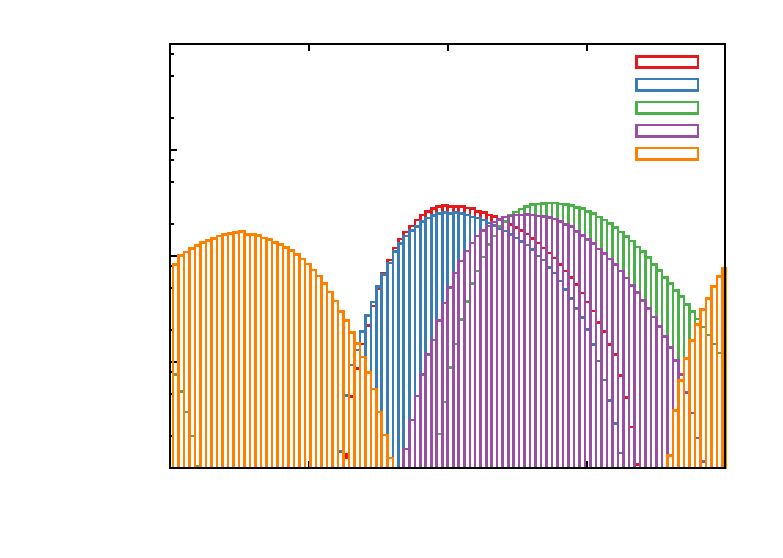
\includegraphics{images/unbound-mass-vs-phi}}%
    \gplfronttext
  \end{picture}%
\endgroup

	\caption[Angular distribution (in $\phi$) of the ejecta]{
		Angular distribution (in $\phi$) of the ejecta 5 ms after merger.  The ejecta spans approximately half of the zonal sky, with an angle of $\Delta \phi \sim (0.99-1.13) \pi$, where M12-M7-S9-SFHo has the smallest arc and M12-M7-S9-FSU21 the widest.
	}
	\label{fig:phihisto}
\end{figure}

\begin{figure}
	\centering
	% GNUPLOT: LaTeX picture with Postscript
\begingroup
  \makeatletter
  \providecommand\color[2][]{%
    \GenericError{(gnuplot) \space\space\space\@spaces}{%
      Package color not loaded in conjunction with
      terminal option `colourtext'%
    }{See the gnuplot documentation for explanation.%
    }{Either use 'blacktext' in gnuplot or load the package
      color.sty in LaTeX.}%
    \renewcommand\color[2][]{}%
  }%
  \providecommand\includegraphics[2][]{%
    \GenericError{(gnuplot) \space\space\space\@spaces}{%
      Package graphicx or graphics not loaded%
    }{See the gnuplot documentation for explanation.%
    }{The gnuplot epslatex terminal needs graphicx.sty or graphics.sty.}%
    \renewcommand\includegraphics[2][]{}%
  }%
  \providecommand\rotatebox[2]{#2}%
  \@ifundefined{ifGPcolor}{%
    \newif\ifGPcolor
    \GPcolortrue
  }{}%
  \@ifundefined{ifGPblacktext}{%
    \newif\ifGPblacktext
    \GPblacktexttrue
  }{}%
  % define a \g@addto@macro without @ in the name:
  \let\gplgaddtomacro\g@addto@macro
  % define empty templates for all commands taking text:
  \gdef\gplbacktext{}%
  \gdef\gplfronttext{}%
  \makeatother
  \ifGPblacktext
    % no textcolor at all
    \def\colorrgb#1{}%
    \def\colorgray#1{}%
  \else
    % gray or color?
    \ifGPcolor
      \def\colorrgb#1{\color[rgb]{#1}}%
      \def\colorgray#1{\color[gray]{#1}}%
      \expandafter\def\csname LTw\endcsname{\color{white}}%
      \expandafter\def\csname LTb\endcsname{\color{black}}%
      \expandafter\def\csname LTa\endcsname{\color{black}}%
      \expandafter\def\csname LT0\endcsname{\color[rgb]{1,0,0}}%
      \expandafter\def\csname LT1\endcsname{\color[rgb]{0,1,0}}%
      \expandafter\def\csname LT2\endcsname{\color[rgb]{0,0,1}}%
      \expandafter\def\csname LT3\endcsname{\color[rgb]{1,0,1}}%
      \expandafter\def\csname LT4\endcsname{\color[rgb]{0,1,1}}%
      \expandafter\def\csname LT5\endcsname{\color[rgb]{1,1,0}}%
      \expandafter\def\csname LT6\endcsname{\color[rgb]{0,0,0}}%
      \expandafter\def\csname LT7\endcsname{\color[rgb]{1,0.3,0}}%
      \expandafter\def\csname LT8\endcsname{\color[rgb]{0.5,0.5,0.5}}%
    \else
      % gray
      \def\colorrgb#1{\color{black}}%
      \def\colorgray#1{\color[gray]{#1}}%
      \expandafter\def\csname LTw\endcsname{\color{white}}%
      \expandafter\def\csname LTb\endcsname{\color{black}}%
      \expandafter\def\csname LTa\endcsname{\color{black}}%
      \expandafter\def\csname LT0\endcsname{\color{black}}%
      \expandafter\def\csname LT1\endcsname{\color{black}}%
      \expandafter\def\csname LT2\endcsname{\color{black}}%
      \expandafter\def\csname LT3\endcsname{\color{black}}%
      \expandafter\def\csname LT4\endcsname{\color{black}}%
      \expandafter\def\csname LT5\endcsname{\color{black}}%
      \expandafter\def\csname LT6\endcsname{\color{black}}%
      \expandafter\def\csname LT7\endcsname{\color{black}}%
      \expandafter\def\csname LT8\endcsname{\color{black}}%
    \fi
  \fi
  \setlength{\unitlength}{0.0500bp}%
  \begin{picture}(7200.00,5040.00)%
    \gplgaddtomacro\gplbacktext{%
      \csname LTb\endcsname%
      \put(1342,704){\makebox(0,0)[r]{\strut{} 1e-05}}%
      \put(1342,1722){\makebox(0,0)[r]{\strut{} 0.0001}}%
      \put(1342,2740){\makebox(0,0)[r]{\strut{} 0.001}}%
      \put(1342,3757){\makebox(0,0)[r]{\strut{} 0.01}}%
      \put(1342,4775){\makebox(0,0)[r]{\strut{} 0.1}}%
      \put(1474,484){\makebox(0,0){\strut{}-1}}%
      \put(2806,484){\makebox(0,0){\strut{}-0.5}}%
      \put(4139,484){\makebox(0,0){\strut{} 0}}%
      \put(5471,484){\makebox(0,0){\strut{} 0.5}}%
      \put(6803,484){\makebox(0,0){\strut{} 1}}%
      \put(176,2739){\rotatebox{-270}{\makebox(0,0){\strut{}$\log_{10}(M_{\rm ej})$ ($M_{\odot}$)}}}%
      \put(4138,154){\makebox(0,0){\strut{}$\cos(\theta)$}}%
    }%
    \gplgaddtomacro\gplfronttext{%
      \csname LTb\endcsname%
      \put(2461,4602){\makebox(0,0)[l]{\strut{}M12-M7-S9-DD2}}%
      \csname LTb\endcsname%
      \put(2461,4382){\makebox(0,0)[l]{\strut{}M14-M7-S9-DD2}}%
      \csname LTb\endcsname%
      \put(2461,4162){\makebox(0,0)[l]{\strut{}M12-M7-S9-FSU21}}%
      \csname LTb\endcsname%
      \put(2461,3942){\makebox(0,0)[l]{\strut{}M14-M7-S9-FSU21}}%
      \csname LTb\endcsname%
      \put(2461,3722){\makebox(0,0)[l]{\strut{}M12-M7-S9-SFHo}}%
    }%
    \gplbacktext
    \put(0,0){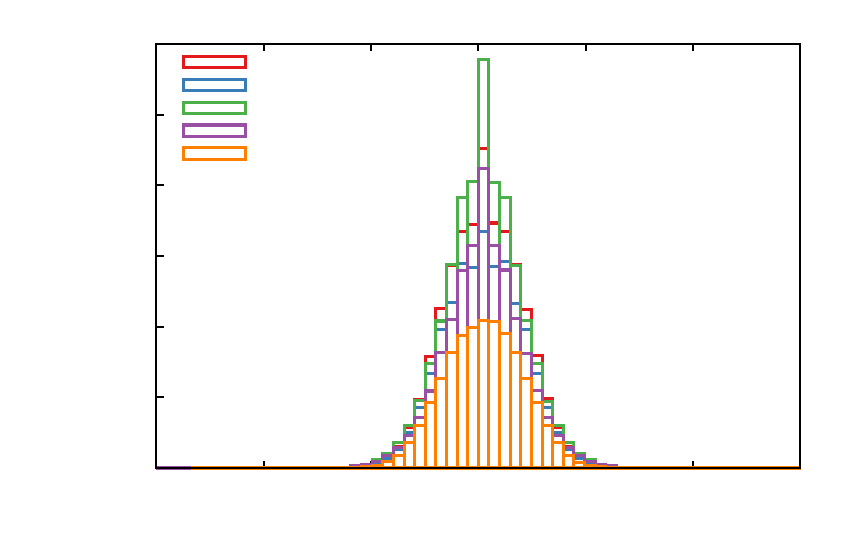
\includegraphics{images/unbound-mass-vs-costheta}}%
    \gplfronttext
  \end{picture}%
\endgroup

	\caption[Angular distribution (in $\theta$) of the ejecta]{
		Angular distribution (in $\theta$) of the ejecta 5 ms after merger.  
		Most of the ejecta matter is constrained around the equator, within $|\theta| \leq \pi/4$ and all of it is constrained with $|\theta| \leq \pi/2$.
	}
	\label{fig:costhetahisto}
\end{figure}


In addition, the ejecta geometry plays an integral role in the kilonova properties, introducing a dependence between the kilonovae signal and the orientation of the binary~\cite{FoucartDD2:2017}.
In Figures \ref{fig:phihisto} and \ref{fig:costhetahisto}, we show the angular distribution of the ejecta in a spherical coordinate system in the inertial frame, where $\cos(\theta) = 0$ corresponds to the equator.  
Our results are consistent with previous black hole-neutron star simulations, where the unbound material forms a crescent with an opening zonal angle $\Delta \phi \sim \pi$ and meridional angle $\Delta \theta \lesssim \pi/4$.
We do not determine an equation of state dependence on the angular speed.


\section{Post-merger remnant: formation of the protodisk and fallback admixture}
\label{sec:disk-analysis}

Accretion of the fluid happens at a maximal rate during the merger. 
Around $\sym 2.5$ ms after merger, this rapid accretion rate onto the black hole begins to slow and the average temperature of the fluid begins to reach a local minimum.
In our simulations, this window was the most difficult epoch of the merger, as the rate of expansion in the tail and then circularization of inflowing gas near the horizon led to the creation of thousands of subdomains
\footnote{
We experienced an overwhelming number of memory issues here, and had to constantly but conservatively increase the number of computer processor cores used in each simulation.
That is, the number of fluid subdomains per processor quickly increased by a factor of (up to) six, requiring diligence in monitoring domain creation and increasing the requisite number of processors to improve the load balancing.
Performance suffers the worst during and shortly after merger, and makes gains as the resolution (i.e. subdomain size) was allowed to be lowered (increased) after maximal accretion and after circularization.  
For example, between the beginning of the plunge and the first derefinement, all simulations required $\sim 450000$ CPU hours to evolve 1 ms of merger (where timesteps shrink to nanoseconds), while the entire duration of the inspiral ($\sim 15 - 20$ ms) was performed with one 10th of this effort. 
}
.
At around the same time, the fluid eventually self-intersects when the higher density thin infalling stream shocks against less dense fluid in the wider part of the stream.
This drives the fluid to slowly circularize into an early-evolution accretion disk, which we call the protodisk.
On the timescale of $\sym (10-20)$ms post-merger, the protodisk continues to accrete gas into the black hole, but also cultivates fallback material from the bound portion of the initially outgoing tail, which contributes to the  amount of dynamical ejecta on much longer timescales on the order of seconds~\cite{Fernandez2013,Just2014}.
The peak of the surface density of the disk begins to gradually advance outwards from the black hole horizon.
The disk secularizes from the tail over this $\sym 10$ms period,
eventually forming an axisymmetric disk that could be evolved on much longer timescales if magnetic effects or an equivalent artificial viscosity scheme to model angular momentum transport were added.

\begin{figure}
	\centering
	% GNUPLOT: LaTeX picture with Postscript
\begingroup
  \makeatletter
  \providecommand\color[2][]{%
    \GenericError{(gnuplot) \space\space\space\@spaces}{%
      Package color not loaded in conjunction with
      terminal option `colourtext'%
    }{See the gnuplot documentation for explanation.%
    }{Either use 'blacktext' in gnuplot or load the package
      color.sty in LaTeX.}%
    \renewcommand\color[2][]{}%
  }%
  \providecommand\includegraphics[2][]{%
    \GenericError{(gnuplot) \space\space\space\@spaces}{%
      Package graphicx or graphics not loaded%
    }{See the gnuplot documentation for explanation.%
    }{The gnuplot epslatex terminal needs graphicx.sty or graphics.sty.}%
    \renewcommand\includegraphics[2][]{}%
  }%
  \providecommand\rotatebox[2]{#2}%
  \@ifundefined{ifGPcolor}{%
    \newif\ifGPcolor
    \GPcolortrue
  }{}%
  \@ifundefined{ifGPblacktext}{%
    \newif\ifGPblacktext
    \GPblacktexttrue
  }{}%
  % define a \g@addto@macro without @ in the name:
  \let\gplgaddtomacro\g@addto@macro
  % define empty templates for all commands taking text:
  \gdef\gplbacktext{}%
  \gdef\gplfronttext{}%
  \makeatother
  \ifGPblacktext
    % no textcolor at all
    \def\colorrgb#1{}%
    \def\colorgray#1{}%
  \else
    % gray or color?
    \ifGPcolor
      \def\colorrgb#1{\color[rgb]{#1}}%
      \def\colorgray#1{\color[gray]{#1}}%
      \expandafter\def\csname LTw\endcsname{\color{white}}%
      \expandafter\def\csname LTb\endcsname{\color{black}}%
      \expandafter\def\csname LTa\endcsname{\color{black}}%
      \expandafter\def\csname LT0\endcsname{\color[rgb]{1,0,0}}%
      \expandafter\def\csname LT1\endcsname{\color[rgb]{0,1,0}}%
      \expandafter\def\csname LT2\endcsname{\color[rgb]{0,0,1}}%
      \expandafter\def\csname LT3\endcsname{\color[rgb]{1,0,1}}%
      \expandafter\def\csname LT4\endcsname{\color[rgb]{0,1,1}}%
      \expandafter\def\csname LT5\endcsname{\color[rgb]{1,1,0}}%
      \expandafter\def\csname LT6\endcsname{\color[rgb]{0,0,0}}%
      \expandafter\def\csname LT7\endcsname{\color[rgb]{1,0.3,0}}%
      \expandafter\def\csname LT8\endcsname{\color[rgb]{0.5,0.5,0.5}}%
    \else
      % gray
      \def\colorrgb#1{\color{black}}%
      \def\colorgray#1{\color[gray]{#1}}%
      \expandafter\def\csname LTw\endcsname{\color{white}}%
      \expandafter\def\csname LTb\endcsname{\color{black}}%
      \expandafter\def\csname LTa\endcsname{\color{black}}%
      \expandafter\def\csname LT0\endcsname{\color{black}}%
      \expandafter\def\csname LT1\endcsname{\color{black}}%
      \expandafter\def\csname LT2\endcsname{\color{black}}%
      \expandafter\def\csname LT3\endcsname{\color{black}}%
      \expandafter\def\csname LT4\endcsname{\color{black}}%
      \expandafter\def\csname LT5\endcsname{\color{black}}%
      \expandafter\def\csname LT6\endcsname{\color{black}}%
      \expandafter\def\csname LT7\endcsname{\color{black}}%
      \expandafter\def\csname LT8\endcsname{\color{black}}%
    \fi
  \fi
  \setlength{\unitlength}{0.0500bp}%
  \begin{picture}(7920.00,5040.00)%
    \gplgaddtomacro\gplbacktext{%
      \csname LTb\endcsname%
      \put(1210,1130){\makebox(0,0)[r]{\strut{} 1e+11}}%
      \put(1210,3166){\makebox(0,0)[r]{\strut{} 1e+12}}%
      \put(1342,484){\makebox(0,0){\strut{} 20}}%
      \put(2029,484){\makebox(0,0){\strut{} 30}}%
      \put(2716,484){\makebox(0,0){\strut{} 40}}%
      \put(3402,484){\makebox(0,0){\strut{} 50}}%
      \put(4089,484){\makebox(0,0){\strut{} 60}}%
      \put(4776,484){\makebox(0,0){\strut{} 70}}%
      \put(5463,484){\makebox(0,0){\strut{} 80}}%
      \put(6149,484){\makebox(0,0){\strut{} 90}}%
      \put(6836,484){\makebox(0,0){\strut{} 100}}%
      \put(7523,484){\makebox(0,0){\strut{} 110}}%
      \put(176,2739){\rotatebox{-270}{\makebox(0,0){\strut{}$\log_{10}(\rho_0) {\rm (cgs)}$}}}%
      \put(4432,154){\makebox(0,0){\strut{}$ R ({\rm km}) $}}%
    }%
    \gplgaddtomacro\gplfronttext{%
      \csname LTb\endcsname%
      \put(6536,4602){\makebox(0,0)[r]{\strut{}M12-M7-S9-DD2}}%
      \csname LTb\endcsname%
      \put(6536,4382){\makebox(0,0)[r]{\strut{}M14-M7-S9-DD2}}%
      \csname LTb\endcsname%
      \put(6536,4162){\makebox(0,0)[r]{\strut{}M12-M7-S9-FSU21}}%
      \csname LTb\endcsname%
      \put(6536,3942){\makebox(0,0)[r]{\strut{}M14-M7-S9-FSU21}}%
      \csname LTb\endcsname%
      \put(6536,3722){\makebox(0,0)[r]{\strut{}M12-M7-S9-SFHo}}%
    }%
    \gplbacktext
    \put(0,0){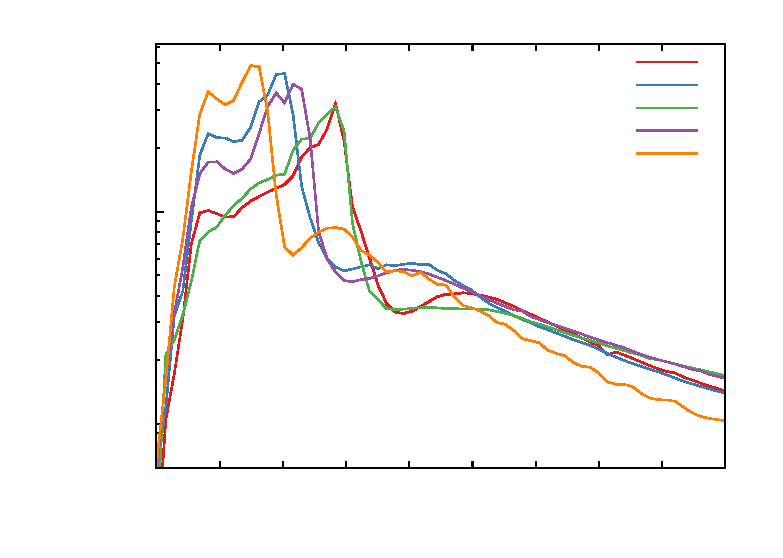
\includegraphics{images/density-of-disk}}%
    \gplfronttext
  \end{picture}%
\endgroup

	\caption[Density profiles of the protodisks 5 ms after merger]{
		Averaged density profiles of the protodisks 5 ms after merger.  The densest zone in the disks ranges $R \sim 30 - 50 {\rm km}$ from the center of the black hole (with a predicted final ISCO radius of $\sym 24 {\rm km}$).  
	}
	\label{fig:diskdensities}
\end{figure}

Because most of our simulations have yet to reach this approximate time of axisymmetrization ($\sym 10$ms post-merger) where one normally measures the properties of the disk, we will at least analyze the protodisk and fallback properties at $5$ms past merger.
The protodisk is a sitinct phase of the evolution and worthy of study in its own right.  
That is, even if we had $100$ms of data, it would still be useful to look at the $5$ms mark.
One argument we can \textit{a priori} make for this is demonstrated in~\cite{Foucart:2014nda}, where simulations with more massive post-merger remnants rapidly form massive, hot inner disks and have less variability during the first $(5-10)$ms, as with ours and in comparison to those with less massive disks yields.
The disk mass predictions of Equation \ref{e:mass_disk} are for the total bound baryonic mass remaining in the system, which include both the protodisk and fallback matter.
We define the disk as the bound matter having a minimum threshold of rotational velocity (i.e., $-1 < v_r/v_\phi < 0$) and a minimum temperature ($T>0.1 {\rm MeV}$ since material shocks when processed into the disk) in order to distinguish the disk from the fallback.
This transition is sharp, with all of the fluid clearly in one mass category or another, and mass counts are insensitive to moderate changes in cutoffs.
The fallback material, by conservation of baryon mass, is then defined as the  remaining bound matter in the tidal tail.
At 5 ms past merger, our simulations yield a wide range of fallback material, in the range of $(32 - 71)\%$ fallback.  
The lowest fallback yield is that of the M12-M7-S9-SFHo model, while both $1.4 M_\odot$ models have the most amount of infalling matter at this time.
This is because more compact stars disrupt closer to the ISCO.

\begin{figure}
	\centering
	% GNUPLOT: LaTeX picture with Postscript
\begingroup
  \makeatletter
  \providecommand\color[2][]{%
    \GenericError{(gnuplot) \space\space\space\@spaces}{%
      Package color not loaded in conjunction with
      terminal option `colourtext'%
    }{See the gnuplot documentation for explanation.%
    }{Either use 'blacktext' in gnuplot or load the package
      color.sty in LaTeX.}%
    \renewcommand\color[2][]{}%
  }%
  \providecommand\includegraphics[2][]{%
    \GenericError{(gnuplot) \space\space\space\@spaces}{%
      Package graphicx or graphics not loaded%
    }{See the gnuplot documentation for explanation.%
    }{The gnuplot epslatex terminal needs graphicx.sty or graphics.sty.}%
    \renewcommand\includegraphics[2][]{}%
  }%
  \providecommand\rotatebox[2]{#2}%
  \@ifundefined{ifGPcolor}{%
    \newif\ifGPcolor
    \GPcolortrue
  }{}%
  \@ifundefined{ifGPblacktext}{%
    \newif\ifGPblacktext
    \GPblacktexttrue
  }{}%
  % define a \g@addto@macro without @ in the name:
  \let\gplgaddtomacro\g@addto@macro
  % define empty templates for all commands taking text:
  \gdef\gplbacktext{}%
  \gdef\gplfronttext{}%
  \makeatother
  \ifGPblacktext
    % no textcolor at all
    \def\colorrgb#1{}%
    \def\colorgray#1{}%
  \else
    % gray or color?
    \ifGPcolor
      \def\colorrgb#1{\color[rgb]{#1}}%
      \def\colorgray#1{\color[gray]{#1}}%
      \expandafter\def\csname LTw\endcsname{\color{white}}%
      \expandafter\def\csname LTb\endcsname{\color{black}}%
      \expandafter\def\csname LTa\endcsname{\color{black}}%
      \expandafter\def\csname LT0\endcsname{\color[rgb]{1,0,0}}%
      \expandafter\def\csname LT1\endcsname{\color[rgb]{0,1,0}}%
      \expandafter\def\csname LT2\endcsname{\color[rgb]{0,0,1}}%
      \expandafter\def\csname LT3\endcsname{\color[rgb]{1,0,1}}%
      \expandafter\def\csname LT4\endcsname{\color[rgb]{0,1,1}}%
      \expandafter\def\csname LT5\endcsname{\color[rgb]{1,1,0}}%
      \expandafter\def\csname LT6\endcsname{\color[rgb]{0,0,0}}%
      \expandafter\def\csname LT7\endcsname{\color[rgb]{1,0.3,0}}%
      \expandafter\def\csname LT8\endcsname{\color[rgb]{0.5,0.5,0.5}}%
    \else
      % gray
      \def\colorrgb#1{\color{black}}%
      \def\colorgray#1{\color[gray]{#1}}%
      \expandafter\def\csname LTw\endcsname{\color{white}}%
      \expandafter\def\csname LTb\endcsname{\color{black}}%
      \expandafter\def\csname LTa\endcsname{\color{black}}%
      \expandafter\def\csname LT0\endcsname{\color{black}}%
      \expandafter\def\csname LT1\endcsname{\color{black}}%
      \expandafter\def\csname LT2\endcsname{\color{black}}%
      \expandafter\def\csname LT3\endcsname{\color{black}}%
      \expandafter\def\csname LT4\endcsname{\color{black}}%
      \expandafter\def\csname LT5\endcsname{\color{black}}%
      \expandafter\def\csname LT6\endcsname{\color{black}}%
      \expandafter\def\csname LT7\endcsname{\color{black}}%
      \expandafter\def\csname LT8\endcsname{\color{black}}%
    \fi
  \fi
  \setlength{\unitlength}{0.0500bp}%
  \begin{picture}(7920.00,5040.00)%
    \gplgaddtomacro\gplbacktext{%
      \csname LTb\endcsname%
      \put(814,704){\makebox(0,0)[r]{\strut{} 0}}%
      \put(814,1286){\makebox(0,0)[r]{\strut{} 2}}%
      \put(814,1867){\makebox(0,0)[r]{\strut{} 4}}%
      \put(814,2449){\makebox(0,0)[r]{\strut{} 6}}%
      \put(814,3030){\makebox(0,0)[r]{\strut{} 8}}%
      \put(814,3612){\makebox(0,0)[r]{\strut{} 10}}%
      \put(814,4193){\makebox(0,0)[r]{\strut{} 12}}%
      \put(814,4775){\makebox(0,0)[r]{\strut{} 14}}%
      \put(946,484){\makebox(0,0){\strut{} 20}}%
      \put(1677,484){\makebox(0,0){\strut{} 30}}%
      \put(2408,484){\makebox(0,0){\strut{} 40}}%
      \put(3138,484){\makebox(0,0){\strut{} 50}}%
      \put(3869,484){\makebox(0,0){\strut{} 60}}%
      \put(4600,484){\makebox(0,0){\strut{} 70}}%
      \put(5331,484){\makebox(0,0){\strut{} 80}}%
      \put(6061,484){\makebox(0,0){\strut{} 90}}%
      \put(6792,484){\makebox(0,0){\strut{} 100}}%
      \put(7523,484){\makebox(0,0){\strut{} 110}}%
      \put(176,2739){\rotatebox{-270}{\makebox(0,0){\strut{}$ T ({\rm MeV}) $}}}%
      \put(4234,154){\makebox(0,0){\strut{}$ R ({\rm km}) $}}%
    }%
    \gplgaddtomacro\gplfronttext{%
      \csname LTb\endcsname%
      \put(6536,4602){\makebox(0,0)[r]{\strut{}M12-M7-S9-DD2}}%
      \csname LTb\endcsname%
      \put(6536,4382){\makebox(0,0)[r]{\strut{}M14-M7-S9-DD2}}%
      \csname LTb\endcsname%
      \put(6536,4162){\makebox(0,0)[r]{\strut{}M12-M7-S9-FSU21}}%
      \csname LTb\endcsname%
      \put(6536,3942){\makebox(0,0)[r]{\strut{}M14-M7-S9-FSU21}}%
      \csname LTb\endcsname%
      \put(6536,3722){\makebox(0,0)[r]{\strut{}M12-M7-S9-SFHo}}%
    }%
    \gplbacktext
    \put(0,0){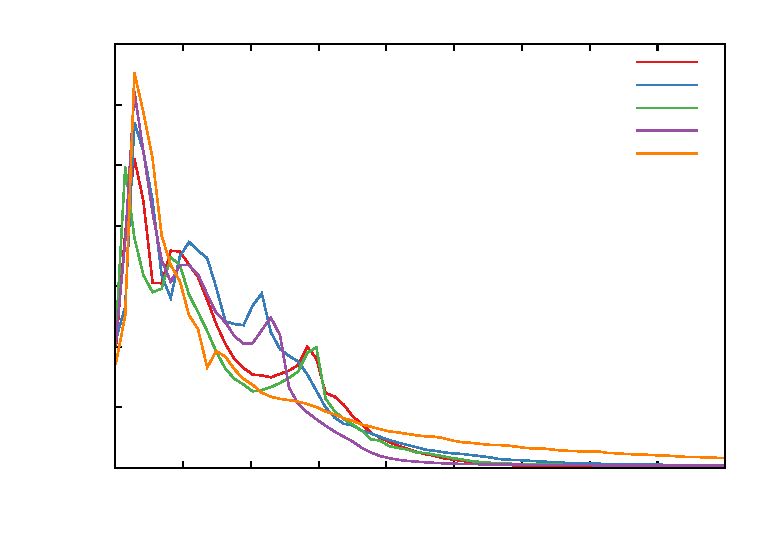
\includegraphics{images/temperature-of-disk}}%
    \gplfronttext
  \end{picture}%
\endgroup

	\caption[Temperature profiles of the protodisks 5 ms after merger]{
		Averaged temperature profiles of the protodisks 5 ms after merger.  The temperature near the peaks of the density profiles is $T \sim (4-7) {\rm MeV}$, and becomes quite cool in the low density region ($r>75 {\rm km}$) outside the disk.  
	}
	\label{fig:disktemps}
\end{figure}

We see that in Figure \ref{fig:diskdensities}, most of the material is within 
$25 {\rm km} < r < 75{\rm km}$ for all models and drops off exponentially after that upper-bound, while the peak of the matter distribution is $r _{\rm disk} \sim (30 - 50) {\rm km}$.  
The composition is roughly constant outside the ISCO, and it is very neutron rich $Y_e \sim 0.05 - 0.08$.  The temperature at the peak of the matter distribution varies as $T \sim (4-7) {\rm MeV}$ between runs, with M12-M7-S9-SFHo having the hottest protodisk and being only slightly more protonized. 
The neutrino luminosities at this time are high, $L_\nu \sim (1.5 - 5.5) \times 10^{53} {\rm egs/s}$, where the less compact M12-M7-S9-DD2 and M12-M7-S9-FSU21 models emit on the lower end, but the more compact models M12-M7-S9-SFHo  and M14-M7-S9-FSU21 are much brighter.
Model M14-M7-S9-DD2 is the brightest in neutrinos.
Most of the emission in all models is in the form of electron anti-neutrinos.


\begin{figure}
	\centering
	% GNUPLOT: LaTeX picture with Postscript
\begingroup
  \makeatletter
  \providecommand\color[2][]{%
    \GenericError{(gnuplot) \space\space\space\@spaces}{%
      Package color not loaded in conjunction with
      terminal option `colourtext'%
    }{See the gnuplot documentation for explanation.%
    }{Either use 'blacktext' in gnuplot or load the package
      color.sty in LaTeX.}%
    \renewcommand\color[2][]{}%
  }%
  \providecommand\includegraphics[2][]{%
    \GenericError{(gnuplot) \space\space\space\@spaces}{%
      Package graphicx or graphics not loaded%
    }{See the gnuplot documentation for explanation.%
    }{The gnuplot epslatex terminal needs graphicx.sty or graphics.sty.}%
    \renewcommand\includegraphics[2][]{}%
  }%
  \providecommand\rotatebox[2]{#2}%
  \@ifundefined{ifGPcolor}{%
    \newif\ifGPcolor
    \GPcolortrue
  }{}%
  \@ifundefined{ifGPblacktext}{%
    \newif\ifGPblacktext
    \GPblacktexttrue
  }{}%
  % define a \g@addto@macro without @ in the name:
  \let\gplgaddtomacro\g@addto@macro
  % define empty templates for all commands taking text:
  \gdef\gplbacktext{}%
  \gdef\gplfronttext{}%
  \makeatother
  \ifGPblacktext
    % no textcolor at all
    \def\colorrgb#1{}%
    \def\colorgray#1{}%
  \else
    % gray or color?
    \ifGPcolor
      \def\colorrgb#1{\color[rgb]{#1}}%
      \def\colorgray#1{\color[gray]{#1}}%
      \expandafter\def\csname LTw\endcsname{\color{white}}%
      \expandafter\def\csname LTb\endcsname{\color{black}}%
      \expandafter\def\csname LTa\endcsname{\color{black}}%
      \expandafter\def\csname LT0\endcsname{\color[rgb]{1,0,0}}%
      \expandafter\def\csname LT1\endcsname{\color[rgb]{0,1,0}}%
      \expandafter\def\csname LT2\endcsname{\color[rgb]{0,0,1}}%
      \expandafter\def\csname LT3\endcsname{\color[rgb]{1,0,1}}%
      \expandafter\def\csname LT4\endcsname{\color[rgb]{0,1,1}}%
      \expandafter\def\csname LT5\endcsname{\color[rgb]{1,1,0}}%
      \expandafter\def\csname LT6\endcsname{\color[rgb]{0,0,0}}%
      \expandafter\def\csname LT7\endcsname{\color[rgb]{1,0.3,0}}%
      \expandafter\def\csname LT8\endcsname{\color[rgb]{0.5,0.5,0.5}}%
    \else
      % gray
      \def\colorrgb#1{\color{black}}%
      \def\colorgray#1{\color[gray]{#1}}%
      \expandafter\def\csname LTw\endcsname{\color{white}}%
      \expandafter\def\csname LTb\endcsname{\color{black}}%
      \expandafter\def\csname LTa\endcsname{\color{black}}%
      \expandafter\def\csname LT0\endcsname{\color{black}}%
      \expandafter\def\csname LT1\endcsname{\color{black}}%
      \expandafter\def\csname LT2\endcsname{\color{black}}%
      \expandafter\def\csname LT3\endcsname{\color{black}}%
      \expandafter\def\csname LT4\endcsname{\color{black}}%
      \expandafter\def\csname LT5\endcsname{\color{black}}%
      \expandafter\def\csname LT6\endcsname{\color{black}}%
      \expandafter\def\csname LT7\endcsname{\color{black}}%
      \expandafter\def\csname LT8\endcsname{\color{black}}%
    \fi
  \fi
  \setlength{\unitlength}{0.0500bp}%
  \begin{picture}(7920.00,5040.00)%
    \gplgaddtomacro\gplbacktext{%
      \csname LTb\endcsname%
      \put(1078,704){\makebox(0,0)[r]{\strut{} 0}}%
      \put(1078,1213){\makebox(0,0)[r]{\strut{} 0.05}}%
      \put(1078,1722){\makebox(0,0)[r]{\strut{} 0.1}}%
      \put(1078,2231){\makebox(0,0)[r]{\strut{} 0.15}}%
      \put(1078,2740){\makebox(0,0)[r]{\strut{} 0.2}}%
      \put(1078,3248){\makebox(0,0)[r]{\strut{} 0.25}}%
      \put(1078,3757){\makebox(0,0)[r]{\strut{} 0.3}}%
      \put(1078,4266){\makebox(0,0)[r]{\strut{} 0.35}}%
      \put(1078,4775){\makebox(0,0)[r]{\strut{} 0.4}}%
      \put(1210,484){\makebox(0,0){\strut{} 20}}%
      \put(1911,484){\makebox(0,0){\strut{} 30}}%
      \put(2613,484){\makebox(0,0){\strut{} 40}}%
      \put(3314,484){\makebox(0,0){\strut{} 50}}%
      \put(4016,484){\makebox(0,0){\strut{} 60}}%
      \put(4717,484){\makebox(0,0){\strut{} 70}}%
      \put(5419,484){\makebox(0,0){\strut{} 80}}%
      \put(6120,484){\makebox(0,0){\strut{} 90}}%
      \put(6822,484){\makebox(0,0){\strut{} 100}}%
      \put(7523,484){\makebox(0,0){\strut{} 110}}%
      \put(176,2739){\rotatebox{-270}{\makebox(0,0){\strut{}$ Y_e $}}}%
      \put(4366,154){\makebox(0,0){\strut{}$ R ({\rm km}) $}}%
    }%
    \gplgaddtomacro\gplfronttext{%
      \csname LTb\endcsname%
      \put(6536,4602){\makebox(0,0)[r]{\strut{}M12-M7-S9-DD2}}%
      \csname LTb\endcsname%
      \put(6536,4382){\makebox(0,0)[r]{\strut{}M14-M7-S9-DD2}}%
      \csname LTb\endcsname%
      \put(6536,4162){\makebox(0,0)[r]{\strut{}M12-M7-S9-FSU21}}%
      \csname LTb\endcsname%
      \put(6536,3942){\makebox(0,0)[r]{\strut{}M14-M7-S9-FSU21}}%
      \csname LTb\endcsname%
      \put(6536,3722){\makebox(0,0)[r]{\strut{}M12-M7-S9-SFHo}}%
    }%
    \gplbacktext
    \put(0,0){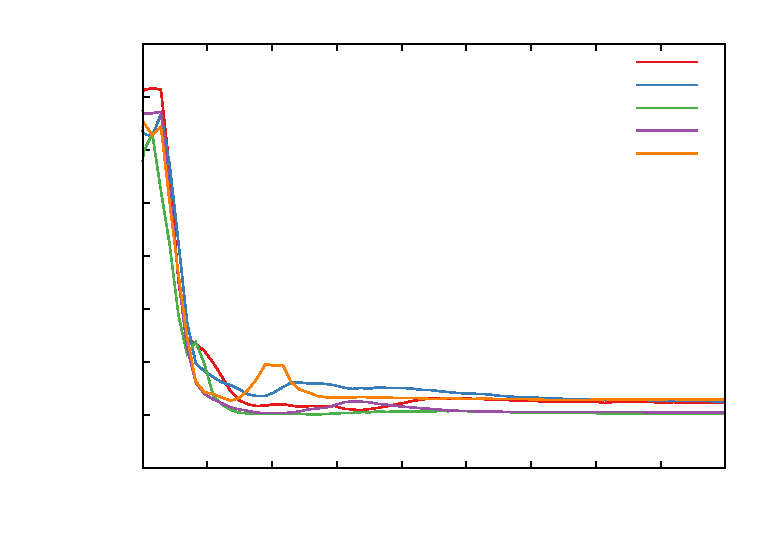
\includegraphics{images/composition-of-disk}}%
    \gplfronttext
  \end{picture}%
\endgroup

	\caption[Radial compositions of the protodisks 5 ms after merger]{
	Averaged radial compositions of the protodisks 5 ms after merger.  
	The fluid is highly protonized ($Ye > 0.25$) near the black hole horizon, while nearly constant in the circularizing portion of the disk ($Y_e \sim 0.05 - 0.08$).
	}
	\label{fig:diskYes}
\end{figure}

%\begin{figure}
%	\centering
%	% GNUPLOT: LaTeX picture with Postscript
\begingroup
  \makeatletter
  \providecommand\color[2][]{%
    \GenericError{(gnuplot) \space\space\space\@spaces}{%
      Package color not loaded in conjunction with
      terminal option `colourtext'%
    }{See the gnuplot documentation for explanation.%
    }{Either use 'blacktext' in gnuplot or load the package
      color.sty in LaTeX.}%
    \renewcommand\color[2][]{}%
  }%
  \providecommand\includegraphics[2][]{%
    \GenericError{(gnuplot) \space\space\space\@spaces}{%
      Package graphicx or graphics not loaded%
    }{See the gnuplot documentation for explanation.%
    }{The gnuplot epslatex terminal needs graphicx.sty or graphics.sty.}%
    \renewcommand\includegraphics[2][]{}%
  }%
  \providecommand\rotatebox[2]{#2}%
  \@ifundefined{ifGPcolor}{%
    \newif\ifGPcolor
    \GPcolortrue
  }{}%
  \@ifundefined{ifGPblacktext}{%
    \newif\ifGPblacktext
    \GPblacktexttrue
  }{}%
  % define a \g@addto@macro without @ in the name:
  \let\gplgaddtomacro\g@addto@macro
  % define empty templates for all commands taking text:
  \gdef\gplbacktext{}%
  \gdef\gplfronttext{}%
  \makeatother
  \ifGPblacktext
    % no textcolor at all
    \def\colorrgb#1{}%
    \def\colorgray#1{}%
  \else
    % gray or color?
    \ifGPcolor
      \def\colorrgb#1{\color[rgb]{#1}}%
      \def\colorgray#1{\color[gray]{#1}}%
      \expandafter\def\csname LTw\endcsname{\color{white}}%
      \expandafter\def\csname LTb\endcsname{\color{black}}%
      \expandafter\def\csname LTa\endcsname{\color{black}}%
      \expandafter\def\csname LT0\endcsname{\color[rgb]{1,0,0}}%
      \expandafter\def\csname LT1\endcsname{\color[rgb]{0,1,0}}%
      \expandafter\def\csname LT2\endcsname{\color[rgb]{0,0,1}}%
      \expandafter\def\csname LT3\endcsname{\color[rgb]{1,0,1}}%
      \expandafter\def\csname LT4\endcsname{\color[rgb]{0,1,1}}%
      \expandafter\def\csname LT5\endcsname{\color[rgb]{1,1,0}}%
      \expandafter\def\csname LT6\endcsname{\color[rgb]{0,0,0}}%
      \expandafter\def\csname LT7\endcsname{\color[rgb]{1,0.3,0}}%
      \expandafter\def\csname LT8\endcsname{\color[rgb]{0.5,0.5,0.5}}%
    \else
      % gray
      \def\colorrgb#1{\color{black}}%
      \def\colorgray#1{\color[gray]{#1}}%
      \expandafter\def\csname LTw\endcsname{\color{white}}%
      \expandafter\def\csname LTb\endcsname{\color{black}}%
      \expandafter\def\csname LTa\endcsname{\color{black}}%
      \expandafter\def\csname LT0\endcsname{\color{black}}%
      \expandafter\def\csname LT1\endcsname{\color{black}}%
      \expandafter\def\csname LT2\endcsname{\color{black}}%
      \expandafter\def\csname LT3\endcsname{\color{black}}%
      \expandafter\def\csname LT4\endcsname{\color{black}}%
      \expandafter\def\csname LT5\endcsname{\color{black}}%
      \expandafter\def\csname LT6\endcsname{\color{black}}%
      \expandafter\def\csname LT7\endcsname{\color{black}}%
      \expandafter\def\csname LT8\endcsname{\color{black}}%
    \fi
  \fi
  \setlength{\unitlength}{0.0500bp}%
  \begin{picture}(7920.00,5040.00)%
    \gplgaddtomacro\gplbacktext{%
      \csname LTb\endcsname%
      \put(1210,704){\makebox(0,0)[r]{\strut{} 0}}%
      \put(1210,1156){\makebox(0,0)[r]{\strut{} 0.002}}%
      \put(1210,1609){\makebox(0,0)[r]{\strut{} 0.004}}%
      \put(1210,2061){\makebox(0,0)[r]{\strut{} 0.006}}%
      \put(1210,2513){\makebox(0,0)[r]{\strut{} 0.008}}%
      \put(1210,2966){\makebox(0,0)[r]{\strut{} 0.01}}%
      \put(1210,3418){\makebox(0,0)[r]{\strut{} 0.012}}%
      \put(1210,3870){\makebox(0,0)[r]{\strut{} 0.014}}%
      \put(1210,4323){\makebox(0,0)[r]{\strut{} 0.016}}%
      \put(1210,4775){\makebox(0,0)[r]{\strut{} 0.018}}%
      \put(1342,484){\makebox(0,0){\strut{} 20}}%
      \put(2029,484){\makebox(0,0){\strut{} 30}}%
      \put(2716,484){\makebox(0,0){\strut{} 40}}%
      \put(3402,484){\makebox(0,0){\strut{} 50}}%
      \put(4089,484){\makebox(0,0){\strut{} 60}}%
      \put(4776,484){\makebox(0,0){\strut{} 70}}%
      \put(5463,484){\makebox(0,0){\strut{} 80}}%
      \put(6149,484){\makebox(0,0){\strut{} 90}}%
      \put(6836,484){\makebox(0,0){\strut{} 100}}%
      \put(7523,484){\makebox(0,0){\strut{} 110}}%
      \put(176,2739){\rotatebox{-270}{\makebox(0,0){\strut{}$ S (k_{\rm B}) $}}}%
      \put(4432,154){\makebox(0,0){\strut{}$ R ({\rm km}) $}}%
    }%
    \gplgaddtomacro\gplfronttext{%
      \csname LTb\endcsname%
      \put(6536,4602){\makebox(0,0)[r]{\strut{}M12-M7-S9-DD2}}%
      \csname LTb\endcsname%
      \put(6536,4382){\makebox(0,0)[r]{\strut{}M14-M7-S9-DD2}}%
      \csname LTb\endcsname%
      \put(6536,4162){\makebox(0,0)[r]{\strut{}M12-M7-S9-FSU21}}%
      \csname LTb\endcsname%
      \put(6536,3942){\makebox(0,0)[r]{\strut{}M14-M7-S9-FSU21}}%
      \csname LTb\endcsname%
      \put(6536,3722){\makebox(0,0)[r]{\strut{}M12-M7-S9-SFHo}}%
    }%
    \gplbacktext
    \put(0,0){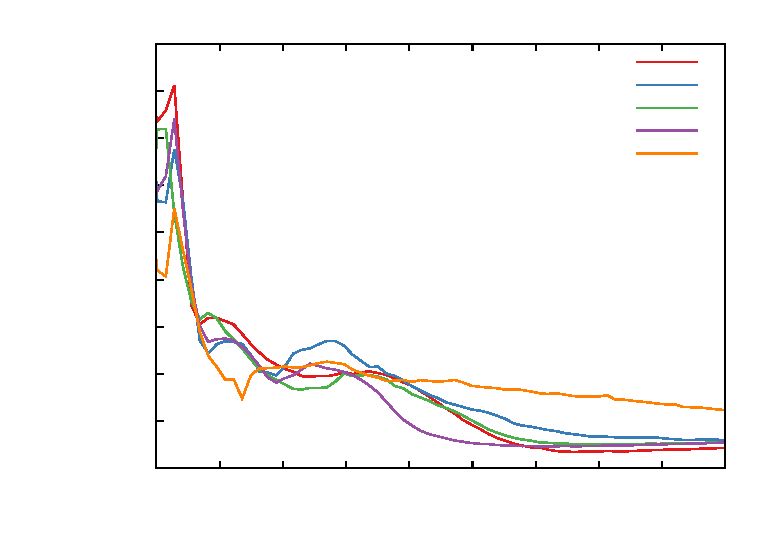
\includegraphics{images/entropy-of-disk}}%
    \gplfronttext
  \end{picture}%
\endgroup

%	\caption[Average entropy of the protodisks 5 ms after merger]{
%		Average entropy of the protodisks 5 ms after merger. \textbf{TODO}
%	}
%	\label{fig:diskentropies}
%\end{figure}

In general, more compact stars led to protodisks that peak in averaged density closer to the black hole, and hotter (Figure \ref{fig:disktemps}).
Since the only difference in our models is compaction (equation of state),
neutron star compactness might be sufficient enough to explain the variability in protodisk structures. 

\subsection{Evolution of the protodisk}

For one model, M12-M7-S9-M12, we evolved the remnant and fluid $\sym 11$ms passed merger time, and are able to track the changes in protodisk structure during peak fallback.
The accretion rate during this time is high $\dot{M}_{\rm BH} \sim 7 M_\odot s^{-1}$, but not as high as the fallback rate of the bound tail onto the disk $\dot{M}_{\rm fall} \sim 17 M_\odot {\rm s}^{-1}$.
We find that the protodisk mass increased $\sym 2 \times 10^{-2} M_\odot$ during the first $5$ms and $8$ms after merger, and $\sym4 \times 10^{-2} M_\odot$ between $8$ms and $11$ms after merger.
We conclude that much of early-formation protodisk material will either accrete onto the black hole or eventually mix with the fallback.
Most of the longterm evolution disk, therefore, will be composed of fallback, as opposed to the initially circulating fluid.

During the fallback time, the disk initially heats up between $(5-8)$ms after merger, and then cools during the $(8-11)$ms interval. 
During the first interval, the fallback is shock-heating the protodisk.
During the second interval, 
as hotter and more protonized fluid is being deposited into the black hole,
the remnant begins to get much smoother in the density profile as the longer-term  accretion disk begins to form.

We think that this distinction between fallback matter and protodisk could be of significant interest, and is worth exploring the nature of the fallback rate between models.
The protodisk is certainly energetic enough to contribute to sGRB's, even ones that occur later on in the evolution.
%The lifespan of a GRB depends on the accretion rate, which, at least in the limit where the accretion timescale is only a function of $\alpha$-viscosity, is on the order of the dynamical timescale of the disk.
%That timescale in turn depends on the height of the disk.
Indeed,~\cite{Aloy:2004nh} determined that SGRBs may last $\sym10$ times longer than the duration of the energy input $L_{\nu \bar{\nu}}$, a timescale of $\sym 10$ms ~\cite{shibata2006magnetized}.
In simulations performed by ~\cite{noori2016dissertation}, accretion disk simulations with fallback seem to suggest including MHD in earlier times is necessary, as the timeframe on which the (proto-)disk cools could be in the ~$(5-20)$ms range.
Neutrinos begin to quickly cool the circulating fluid if there's no heating from shocks (fallback) or magnetic turbulence (MRI), so the matter begins to lose its ability to transport angular momentum, and therefore accrete.

Including Lagrangian tracers in the evolution of the fallback material could provide an estimate for the amount of matter that remains in the later-time, axisymmetric disk from the primordial circularizing remnant.
In~\cite{FoucartDD2:2017}, we collected the ballistic trajectories of the outflowing particles in order to determine the asymptotic velocities.
Likewise, a similar processing of our data could do this for following the bound material.
Tracking the trajectories from bound-particle Keplerian velocities will give us a measure of the fallback rate over time.

\begin{figure}
	\centering
	% GNUPLOT: LaTeX picture with Postscript
\begingroup
  \makeatletter
  \providecommand\color[2][]{%
    \GenericError{(gnuplot) \space\space\space\@spaces}{%
      Package color not loaded in conjunction with
      terminal option `colourtext'%
    }{See the gnuplot documentation for explanation.%
    }{Either use 'blacktext' in gnuplot or load the package
      color.sty in LaTeX.}%
    \renewcommand\color[2][]{}%
  }%
  \providecommand\includegraphics[2][]{%
    \GenericError{(gnuplot) \space\space\space\@spaces}{%
      Package graphicx or graphics not loaded%
    }{See the gnuplot documentation for explanation.%
    }{The gnuplot epslatex terminal needs graphicx.sty or graphics.sty.}%
    \renewcommand\includegraphics[2][]{}%
  }%
  \providecommand\rotatebox[2]{#2}%
  \@ifundefined{ifGPcolor}{%
    \newif\ifGPcolor
    \GPcolortrue
  }{}%
  \@ifundefined{ifGPblacktext}{%
    \newif\ifGPblacktext
    \GPblacktexttrue
  }{}%
  % define a \g@addto@macro without @ in the name:
  \let\gplgaddtomacro\g@addto@macro
  % define empty templates for all commands taking text:
  \gdef\gplbacktext{}%
  \gdef\gplfronttext{}%
  \makeatother
  \ifGPblacktext
    % no textcolor at all
    \def\colorrgb#1{}%
    \def\colorgray#1{}%
  \else
    % gray or color?
    \ifGPcolor
      \def\colorrgb#1{\color[rgb]{#1}}%
      \def\colorgray#1{\color[gray]{#1}}%
      \expandafter\def\csname LTw\endcsname{\color{white}}%
      \expandafter\def\csname LTb\endcsname{\color{black}}%
      \expandafter\def\csname LTa\endcsname{\color{black}}%
      \expandafter\def\csname LT0\endcsname{\color[rgb]{1,0,0}}%
      \expandafter\def\csname LT1\endcsname{\color[rgb]{0,1,0}}%
      \expandafter\def\csname LT2\endcsname{\color[rgb]{0,0,1}}%
      \expandafter\def\csname LT3\endcsname{\color[rgb]{1,0,1}}%
      \expandafter\def\csname LT4\endcsname{\color[rgb]{0,1,1}}%
      \expandafter\def\csname LT5\endcsname{\color[rgb]{1,1,0}}%
      \expandafter\def\csname LT6\endcsname{\color[rgb]{0,0,0}}%
      \expandafter\def\csname LT7\endcsname{\color[rgb]{1,0.3,0}}%
      \expandafter\def\csname LT8\endcsname{\color[rgb]{0.5,0.5,0.5}}%
    \else
      % gray
      \def\colorrgb#1{\color{black}}%
      \def\colorgray#1{\color[gray]{#1}}%
      \expandafter\def\csname LTw\endcsname{\color{white}}%
      \expandafter\def\csname LTb\endcsname{\color{black}}%
      \expandafter\def\csname LTa\endcsname{\color{black}}%
      \expandafter\def\csname LT0\endcsname{\color{black}}%
      \expandafter\def\csname LT1\endcsname{\color{black}}%
      \expandafter\def\csname LT2\endcsname{\color{black}}%
      \expandafter\def\csname LT3\endcsname{\color{black}}%
      \expandafter\def\csname LT4\endcsname{\color{black}}%
      \expandafter\def\csname LT5\endcsname{\color{black}}%
      \expandafter\def\csname LT6\endcsname{\color{black}}%
      \expandafter\def\csname LT7\endcsname{\color{black}}%
      \expandafter\def\csname LT8\endcsname{\color{black}}%
    \fi
  \fi
  \setlength{\unitlength}{0.0500bp}%
  \begin{picture}(7200.00,5040.00)%
    \gplgaddtomacro\gplbacktext{%
      \csname LTb\endcsname%
      \put(814,704){\makebox(0,0)[r]{\strut{} 0}}%
      \put(814,1286){\makebox(0,0)[r]{\strut{} 2}}%
      \put(814,1867){\makebox(0,0)[r]{\strut{} 4}}%
      \put(814,2449){\makebox(0,0)[r]{\strut{} 6}}%
      \put(814,3030){\makebox(0,0)[r]{\strut{} 8}}%
      \put(814,3612){\makebox(0,0)[r]{\strut{} 10}}%
      \put(814,4193){\makebox(0,0)[r]{\strut{} 12}}%
      \put(814,4775){\makebox(0,0)[r]{\strut{} 14}}%
      \put(946,484){\makebox(0,0){\strut{} 20}}%
      \put(1597,484){\makebox(0,0){\strut{} 30}}%
      \put(2248,484){\makebox(0,0){\strut{} 40}}%
      \put(2898,484){\makebox(0,0){\strut{} 50}}%
      \put(3549,484){\makebox(0,0){\strut{} 60}}%
      \put(4200,484){\makebox(0,0){\strut{} 70}}%
      \put(4851,484){\makebox(0,0){\strut{} 80}}%
      \put(5501,484){\makebox(0,0){\strut{} 90}}%
      \put(6152,484){\makebox(0,0){\strut{} 100}}%
      \put(6803,484){\makebox(0,0){\strut{} 110}}%
      \put(176,2739){\rotatebox{-270}{\makebox(0,0){\strut{}$ T ({\rm MeV}) $}}}%
      \put(3874,154){\makebox(0,0){\strut{}$ R ({\rm km}) $}}%
    }%
    \gplgaddtomacro\gplfronttext{%
      \csname LTb\endcsname%
      \put(5816,4602){\makebox(0,0)[r]{\strut{}5ms}}%
      \csname LTb\endcsname%
      \put(5816,4382){\makebox(0,0)[r]{\strut{}8ms}}%
      \csname LTb\endcsname%
      \put(5816,4162){\makebox(0,0)[r]{\strut{}11ms}}%
    }%
    \gplbacktext
    \put(0,0){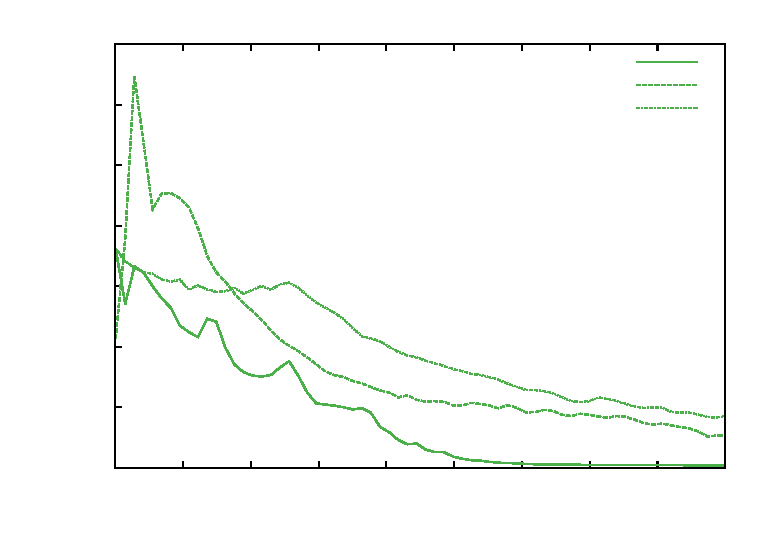
\includegraphics{images/long-temperature-of-disk}}%
    \gplfronttext
  \end{picture}%
\endgroup

	\caption[Average temperature of the protodisks 5, 8, and 11 ms after merger]{
		Average temperature of the protodisk 5, 8, and 11 ms after merger in model M12-M7-S9-FSU21.
	}
	\label{fig:longdiskentropies}
\end{figure}

\textit{To my committee: we are currently working on this technique and should have it included in the final draft of this manuscript.  I will also be adding some multi-dimensional profiles in $\rho_0$, $Y_e$, and $T$ for this case, particularly to show the spread of the radius of densest point and the deposition of highly protonized matter onto the black hole.}


\section{Discussion}
\label{sec:discussion}

The first simulations of neutron stars with multiple hot, composition-dependent nuclear theory-based equations of state in black hole-neutron star mergers using a general relativistic fluid code were performed in this study.  
The mergers presented here all consider the same black hole parameters, with an orbitally aligned, relatively high black hole spin $\chi_{\rm BH} = 0.9$ and  mass $M_{\rm BH} = 7 M_\odot$, within the range of the most likely black hole masses.  
The neutron stars considered in this paper were evolved with the SFHo, DD2 and FSU2.1 equations of state with relatively average masses $M_{\rm NS} = (1.2,1.4) M_\odot$ over a range of compactnesess.  
These equations of state satisfy a number of observational, experimental and causal constraints.  
The ejecta of the five models that evolved far enough passed merger ($t - t_{\rm merger} \sim 3$ms) is very neutron-rich $Y_e = 0.05$, allowing for the robust production of heavy elements on the 2nd and 3rd peak of r-process nucleosynthesis.
Comparing with previous results in the literature, we do no find much distinction in the crescent size and localization of the ejecta between models that cannot adequately be understood by compactness alone.  The composition of the ejecta is all roughly the same, i.e. very neutron rich $Y_e \sim 0.05$, just $5$ms after merger, with a high, average velocity similar to the predicted value for $q=7$ systems, $\langle v \rangle_{\rm ej} \sim 0.2 c$.

We note that while we have implemented our improved algorithm to selectively evolve only non-vacuum subdomains on the finite volume grid, three of our models (M14-M17-S9-SFHo, M12-M17-S9-SFHx, and M14-M17-S9-SFHx) still had significant numerical error during merger. 
This is because our hot, composition-dependent, tidally-disrupting material forms a much narrower tidal tail than other piecewise polytrope models.
An improvement to our algorithm would be to allow true adaptive mesh refinement, so that evolution subdomains could themselves shrink and expand given the average density gradient of the material inside.
The ejecta has an average velocity consistent with the prediction of the fitting formulae, and a measured mass that is somewhat consistent with the predicted values.
Two of the models predicted masses outside the relative error range $\sym20\%$ from the results of the experiment.
The discrepancies appear in both least compact model M12-M7-S9-FSU21 and in the most compact model M14-M7-S9-DD2.
We find that the fitting-formula prescription for the ejecta mass from Version 2 of the~\cite{Kyutoku:2015} paper was better than the updated Version 3 of the paper, and have chosen to display the ``v2'' predictions in Table \ref{tab:results}.

We find that the protodisk and fallback physics might be a worthwhile investigation into the origins of accretion disk GRB's.
The protodisk phase is certainly the most energetic phase of the post-merger evolution, which is emitting a lot of energy in the form of electron neutrinos and antineutrinos. 
The accretion rate for our long-term evolution study of the protodisk remains high in the first $(5-8)$ms after merger ($\dot{M}^{5-8 {\rm ms}}_{\rm BH} \sim 5 M_\odot s^{-1}$), but as the fallback rate begins to increase, this drives heating via shocks, transporting angular momentum through an even higher rate of accretion onto the black hole ($\dot{M}^{8-11 {\rm ms}}_{\rm BH} \sim 10 M_\odot s^{-1}$).
Presumably, this is because the flow is extremely nonaxisymmetric at this point, so we do not need an ``effective viscosity'' to enable accretion.
The average fallback rate during each of these intervals is almost twice as high as the accretion rate.
It would be interesting to learn what percentage of fluid elements from the accretion disks were once protodisk.
At $5$ms passed merger, depending on how closely the star disrupts to the ISCO (determined both by compactness and the mass-ratio), roughly half of the bound matter remaining in the system is fallback.

As to the initial curiosity of what features the hot equations of state might imprint, we find that different models do affect ejecta mass, but only in ways captured by cold models, and does not affect the spread of the ejecta or composition in interesting ways.
However, different equation of state models do affect the protodisk properties, such as disk size and mass, neutrino luminosity and fallback time, although only via variance in compaction.
 

\paragraph{In-progress work}

We are performing code-validation for two of our runs using a $\sym\,125\%$ grid-spacing of that used in our work.
We are also attempting to get at least one of our more troublesome models evolving again, by globally increasing resolution on the finite volume grid.
There are a number of automation tasks left to do for the Hydro-AMR algorithm, chiefly: automating the process of derefining the innermost levels of the grid at the appropriate time.
Since this project began (it began before Hydro-AMR was available), we have made progress in most of the automation tasks. For example:
(1) re-centering the grid before merger to collocate with the horizon center, 
(2) automating fluid-evolution checkpoint cleaning, 
(3) developing a set of scripts that allow for the easier monitoring and visualization of the simulation volume data, 
and (4) building a set of modular visualization tools for joining and monitoring columnated data.
The calculation of the gravitational waveform is in progress.
One simplification to the post-merger system is to  we are going to do is to turn off the fluid evolution and evolve only the metric quantities until the the waves propogate out to infinity.

\paragraph{Future work} 

For the neutrino emission, we did not include the effects of radiation transport in our simulations, which cannot be determined by the relatively simple neutrino leakage scheme used in this work.
In order to capture an estimate of the production of electron-positron pairs in neutrino-driven winds near the spin axes of the black hole, evolving the fluid with a neutrino radiation code would improve the post-merger remnant evolution.
That is to say, there would be some effect from neutrino absorbtions on the fluid---especially by increasing the $Y_e$ in low-density regions and reducing temperature gradients.
A neutrino transport or ray tracing calculation accompanying the simulations is needed to predict the neutrino annihilation energy deposition rate from the existing disk.
Furthermore, the effects of magnetic fields on the disk contribute heating through MRI turbulence.
Simulations of the longer-lasting post-merger disk would require the inclusion of magnetohydrodynamics or an equivalent artificial viscosity scheme. 
Lastly, if the protodisk phase is important, then it would be useful to develop models of the essential physics of accretion disks undergoing massive infusion from one-arm fallback.

